\documentclass{article}

\usepackage{microtype}
\usepackage{graphicx}
\usepackage{subfigure}
\usepackage{booktabs} % NOTE: for professional tables
\usepackage{makecell}
\usepackage{listings}
\usepackage{xcolor}
\lstset{
  breaklines=true,              % NOTE: enable automatic line breaking
  basicstyle=\small\ttfamily,   % NOTE: adjust the font size and type
  escapeinside={||},            % NOTE: define escape characters for LaTeX commands
}
\usepackage{fancyvrb}
\usepackage{minted}
% Set options for minted:
\setminted{
  breaklines=true,   % Enable automatic line breaking
  fontsize=\small,   % Adjust the font size if needed
  escapeinside=||,
  % Any other options you need
}
\usepackage{mdframed}


\usepackage{lipsum}
\usepackage{listings}
% Rename "Listing: " to "Extract: "
\renewcommand{\lstlistingname}{Extract}

\usepackage{hyperref}


% NOTE: make hyperref and algorithmic work together better:
\newcommand{\theHalgorithm}{\arabic{algorithm}}

% \usepackage{icml2025} % NOTE: will display the line numbers
\usepackage[accepted]{./settings/icml2025} % NOTE: won't display the line numbers
% \usepackage[nohyperref, accepted]{icml2025} % NOTE: won't display the line numbers

% For theorems and such
\usepackage{amsmath}
\usepackage{amssymb}
\usepackage{mathtools}
\usepackage{amsthm}

% if you use cleveref..
\usepackage[capitalize,noabbrev]{cleveref}

%%%%%%%%%%%%%%%%%%%%%%%%%%%%%%%%
% THEOREMS
%%%%%%%%%%%%%%%%%%%%%%%%%%%%%%%%
\theoremstyle{plain}
\newtheorem{theorem}{Theorem}[section]
\newtheorem{proposition}[theorem]{Proposition}
\newtheorem{lemma}[theorem]{Lemma}
\newtheorem{corollary}[theorem]{Corollary}
\theoremstyle{definition}
\newtheorem{definition}[theorem]{Definition}
\newtheorem{assumption}[theorem]{Assumption}
\theoremstyle{remark}
\newtheorem{remark}[theorem]{Remark}

% TODO: is useful during development; simply uncomment the next line
%    and comment out the line below the next line to turn off comments
%\usepackage[disable,textsize=tiny]{todonotes}
\usepackage[textsize=tiny]{todonotes}

\usepackage{multirow}
\usepackage{multicol}
\usepackage{enumitem}
% c.f. Efficient Online Reinforcement Learning Fine-Tuning Need Not Retain Offline Data
\usepackage[most,skins,theorems]{tcolorbox}
\tcbset{
  aibox/.style={
    width=\linewidth,
    top=8pt,
    bottom=4pt,
    colback=blue!6!white,
    colframe=black,
    colbacktitle=black,
    enhanced,
    center,
    attach boxed title to top left={yshift=-0.1in,xshift=0.15in},
    boxed title style={boxrule=0pt,colframe=white,},
  }
}

\newtcolorbox{AIbox}[2][]{aibox,title=#2,#1}

\usepackage[utf8]{inputenc}
\usepackage{listings}

% TODO: remove it in case of problem cuz idk what it do
% \raggedbottom % NOTE: apparently when disabled latex will try to stretch the page's content to the bottom in order to fill the whole page

% \bibliography{reference}
% \bibliographystyle{icml2025}

\usepackage{tabularx} % Add this in your preamble

\begin{document}

\begin{center}
    \begin{minipage}{0.3\textwidth}
        \centering
        
\includegraphics[width=0.8\textwidth]{assets/logos/cristal-lab-black.logo.png}
    \end{minipage}
    \begin{minipage}{0.3\textwidth}
        \centering
        
\includegraphics[width=0.8\textwidth]{assets/logos/universite-lille.logo.png}
    \end{minipage}
    \begin{minipage}{0.3\textwidth}
        \centering
        
\includegraphics[width=0.8\textwidth]{assets/logos/universite-rouen.logo.png}
    \end{minipage}
\end{center}

\vskip 0.75cm

\icmltitlerunning{Bouldering Video Segmentation}
\icmltitle{Bouldering Video Segmentation \\ \large\textit{M1 Data Science Research Project}}

\icmlsetsymbol{equal}{*}

\begin{icmlauthorlist}
\icmlauthor{Nadir Kichou}{ul}
\icmlauthor{Jérémie Boulanger}{sigma}
\icmlauthor{Ludivine Plumhans}{ur}
\icmlauthor{Ludovic Seifert}{ur}
\end{icmlauthorlist}

\icmlaffiliation{ul}{Université de Lille}
\icmlaffiliation{sigma}{CRIStAL Lab, SIGMA}
\icmlaffiliation{ur}{Université de Rouen}

\icmlcorrespondingauthor{Nadir Kichou}{nadir.kichou.etu@univ-lille.fr}

\icmlkeywords{Temporal Action Segmnetation, TAS, Video Machine Learning, Machine Learning, ICML}

\vskip 0.75cm

\newpage

\begin{abstract}
\lipsum[1-2]
\end{abstract}

\section{Introduction}

Here we are going to provide the essential background information.

\todo[inline]{This section might be removed as since we are in report mode and not research mode, we might not need to provide the background information or at least not this early in the report.}

\todo[inline]{Talk about the fact that the data quality is the most important thing and maybe even more important than the model architecture and size and dataset size.}

\todo[inline]{Maybe merge this section with the context.}
\section{Context}
\label{section:context}

\noindent\textbf{Bouldering Basics.} 
It is a form of rock climbing where climbers tackle short but challenging routes, typically lasting around 4 minutes. During this time, climbers have the freedom to choose their climbing strategies, retry as many times as needed, and aim to complete the route as quickly as possible. The ultimate goal is to reach the top of the climb in the least amount of time.

\noindent\textbf{Project Overview.} 
This research project is part of a larger initiative (ANR) aimed at improving bouldering performance. The focus is on developing tools for coaches to analyze bouldering performances, allowing them to provide better advice to help climbers improve.

\noindent\textbf{Existing Tools.} 
Among these tools are: Grip Detection, Path Tracking, Performance Analysis, and more. Several models have already been developed as part of this broader effort, including a model for detecting the grips used by the climber and another for tracking the climber's path during a climb.

\noindent\textbf{Phase Identification.} 
These models provide valuable data, but in order to fully analyze a climber's performance, it is essential to distinguish between the different phases of a bouldering event (Climbing, Observing, Brushing). By doing so, we can apply the appropriate model to each phase and gather the corresponding statistics.

\noindent\textbf{Research Focus.} 
This brings us to my current research project. I will be focusing on Temporal Action Segmentation (TAS), a technique that will allow us to run the grip and path analysis models at the correct timestamps. This step is crucial for gaining deeper insights into the different phases of climbing, such as observing, reading the route, and brushing the grips. By analyzing the durations, order, and impact of these phases on a climber's final performance, we can provide more precise guidance to coaches and improve training methods.

\begin{figure*}[t]
    \centering
    \begin{tabular}{@{}c@{\hspace{15pt}}c@{\hspace{15pt}}c@{\hspace{15pt}}c@{}}
      \setlength{\fboxsep}{0pt}
      \fbox{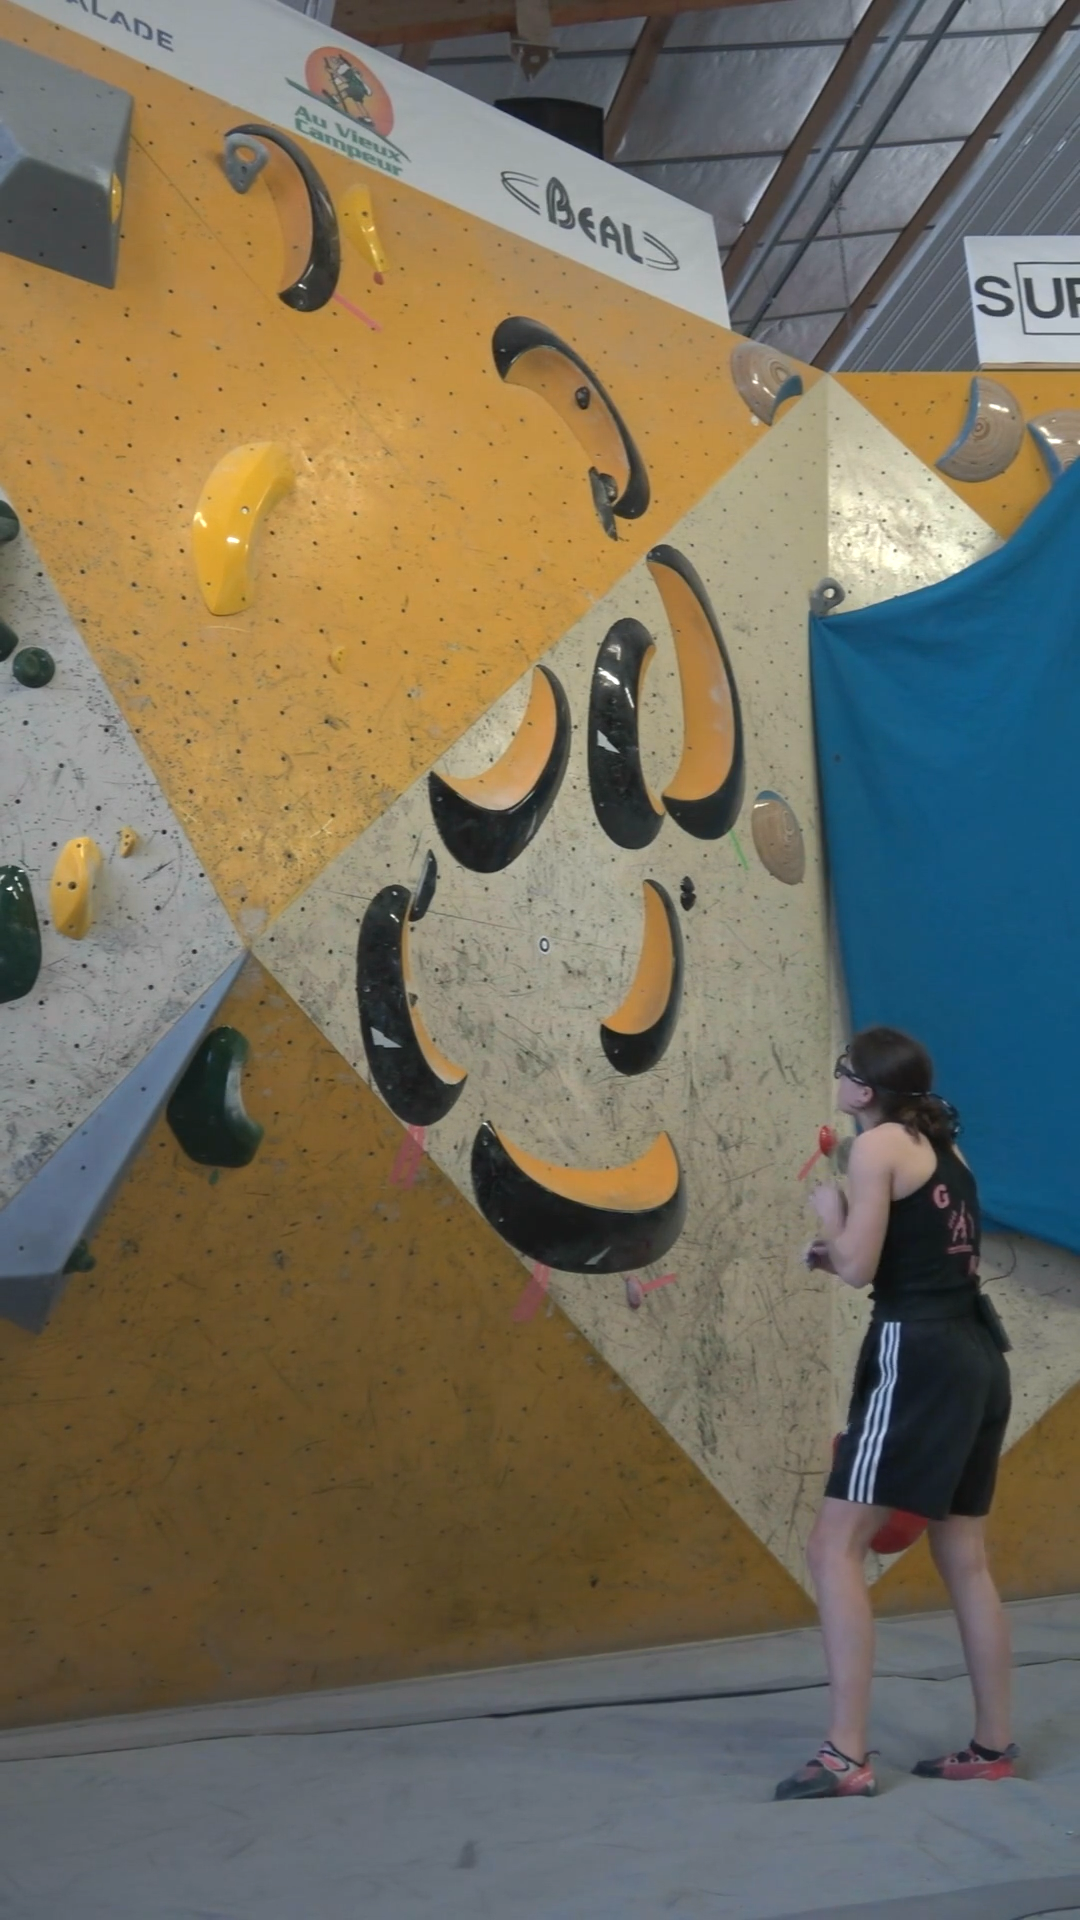
\includegraphics[width=0.2\textwidth]{assets/images/observing.2.png}} &
      \setlength{\fboxsep}{0pt}
      \fbox{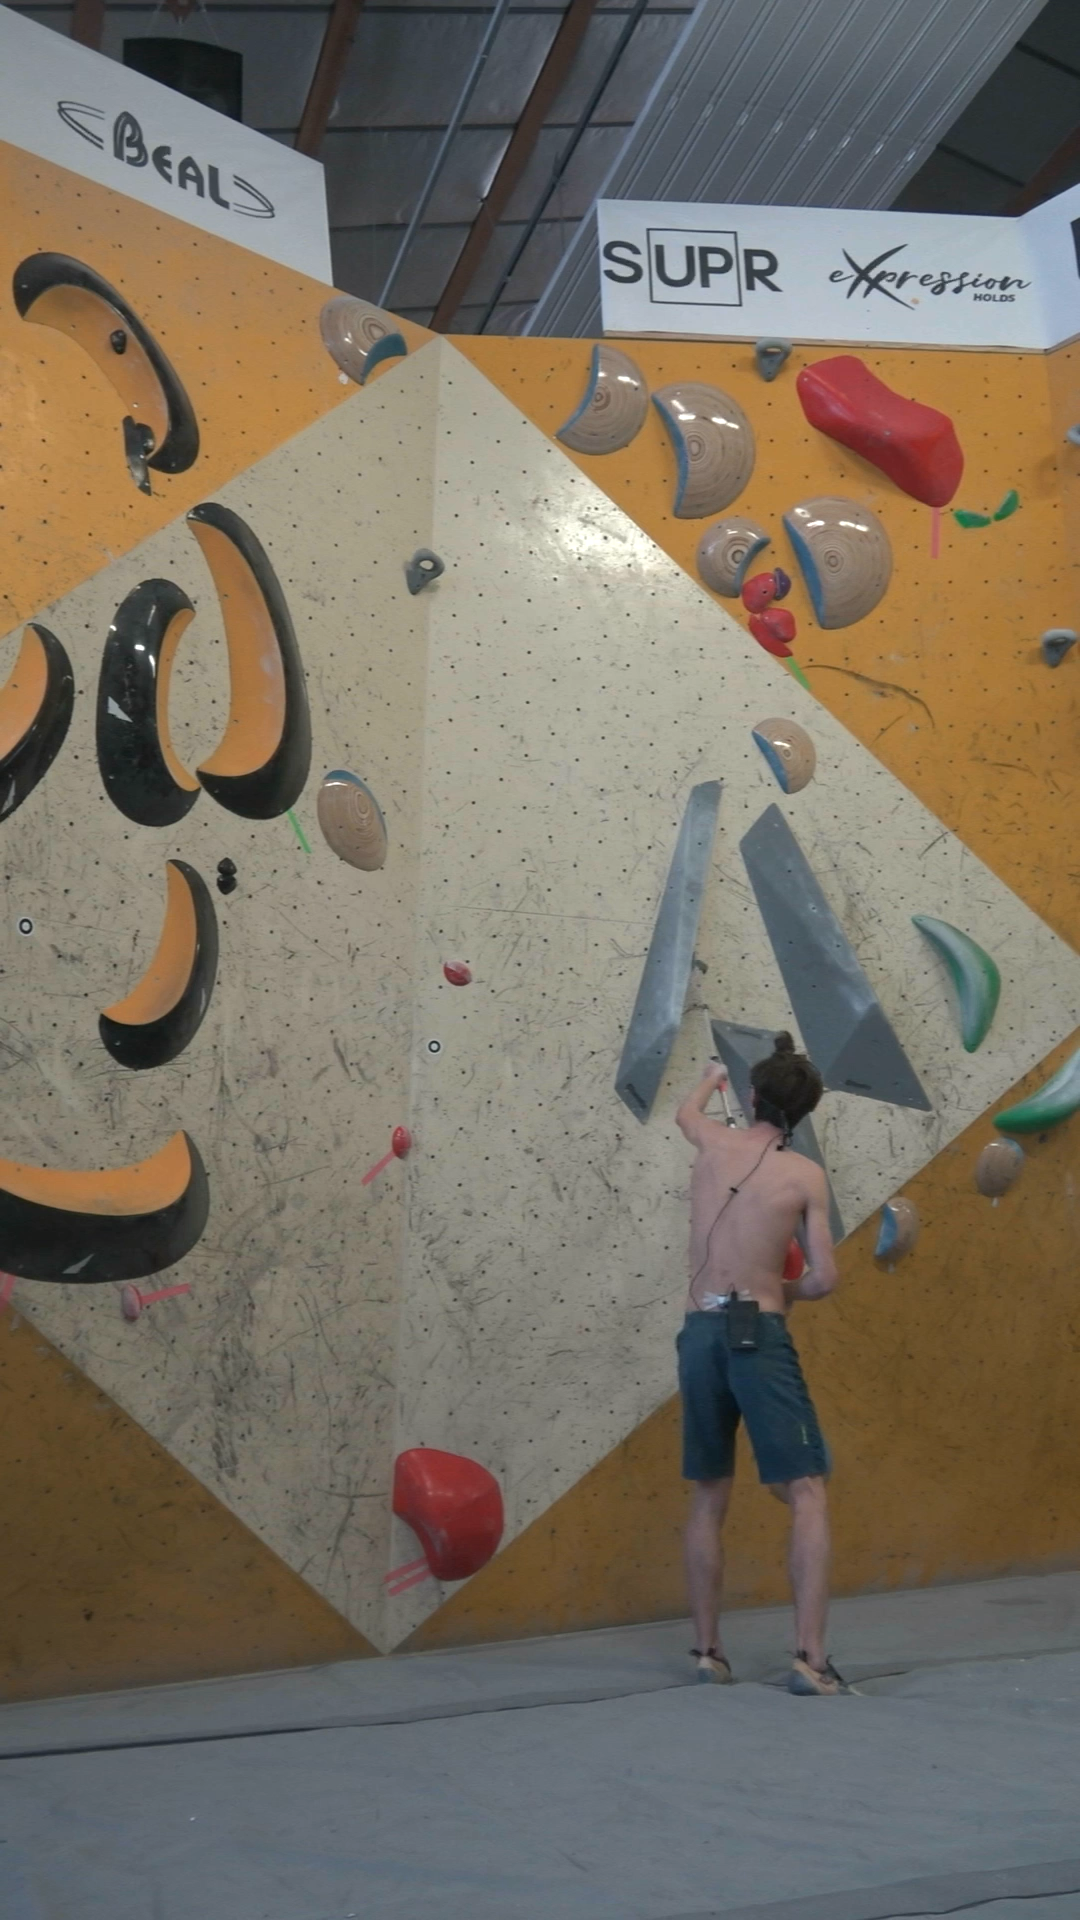
\includegraphics[width=0.2\textwidth]{assets/images/brushing.3.png}} &
      \setlength{\fboxsep}{0pt}
      \fbox{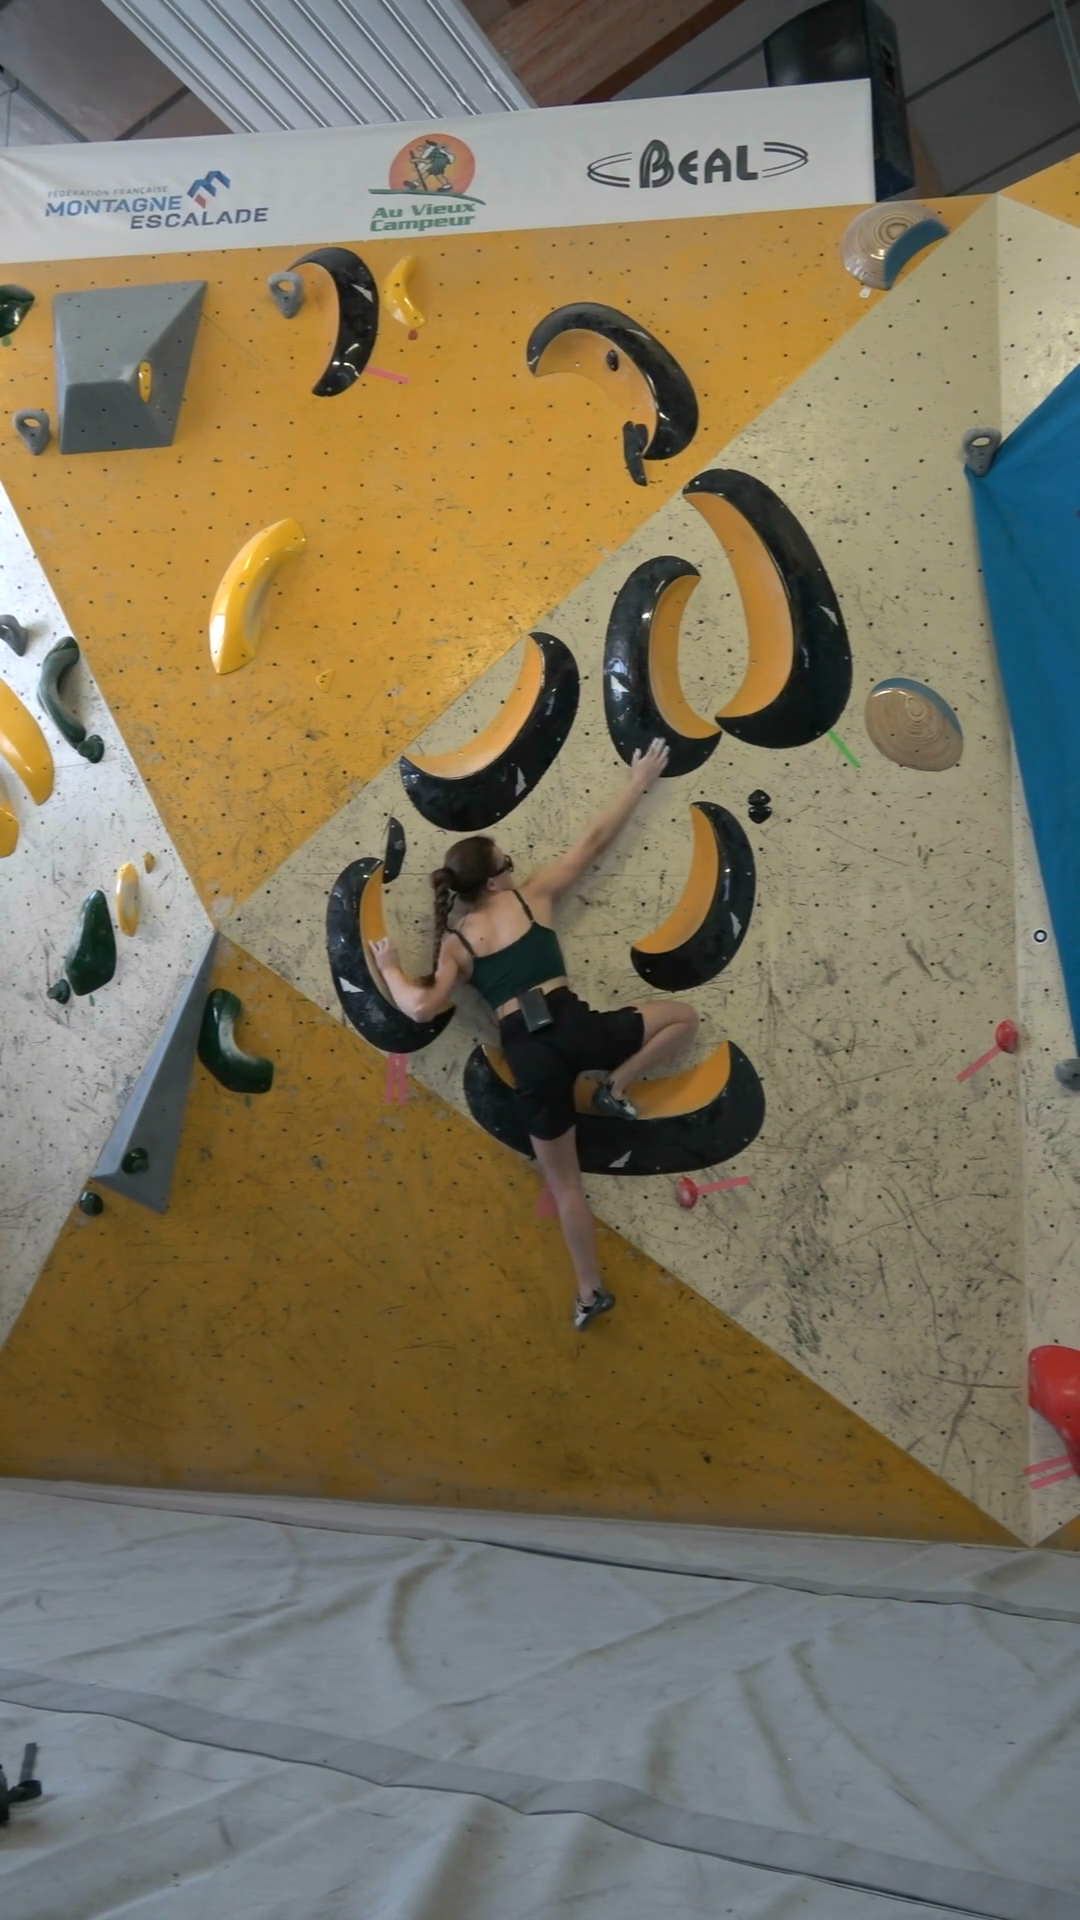
\includegraphics[width=0.2\textwidth]{assets/images/climbing.1.png}} &
      \setlength{\fboxsep}{0pt}
      \fbox{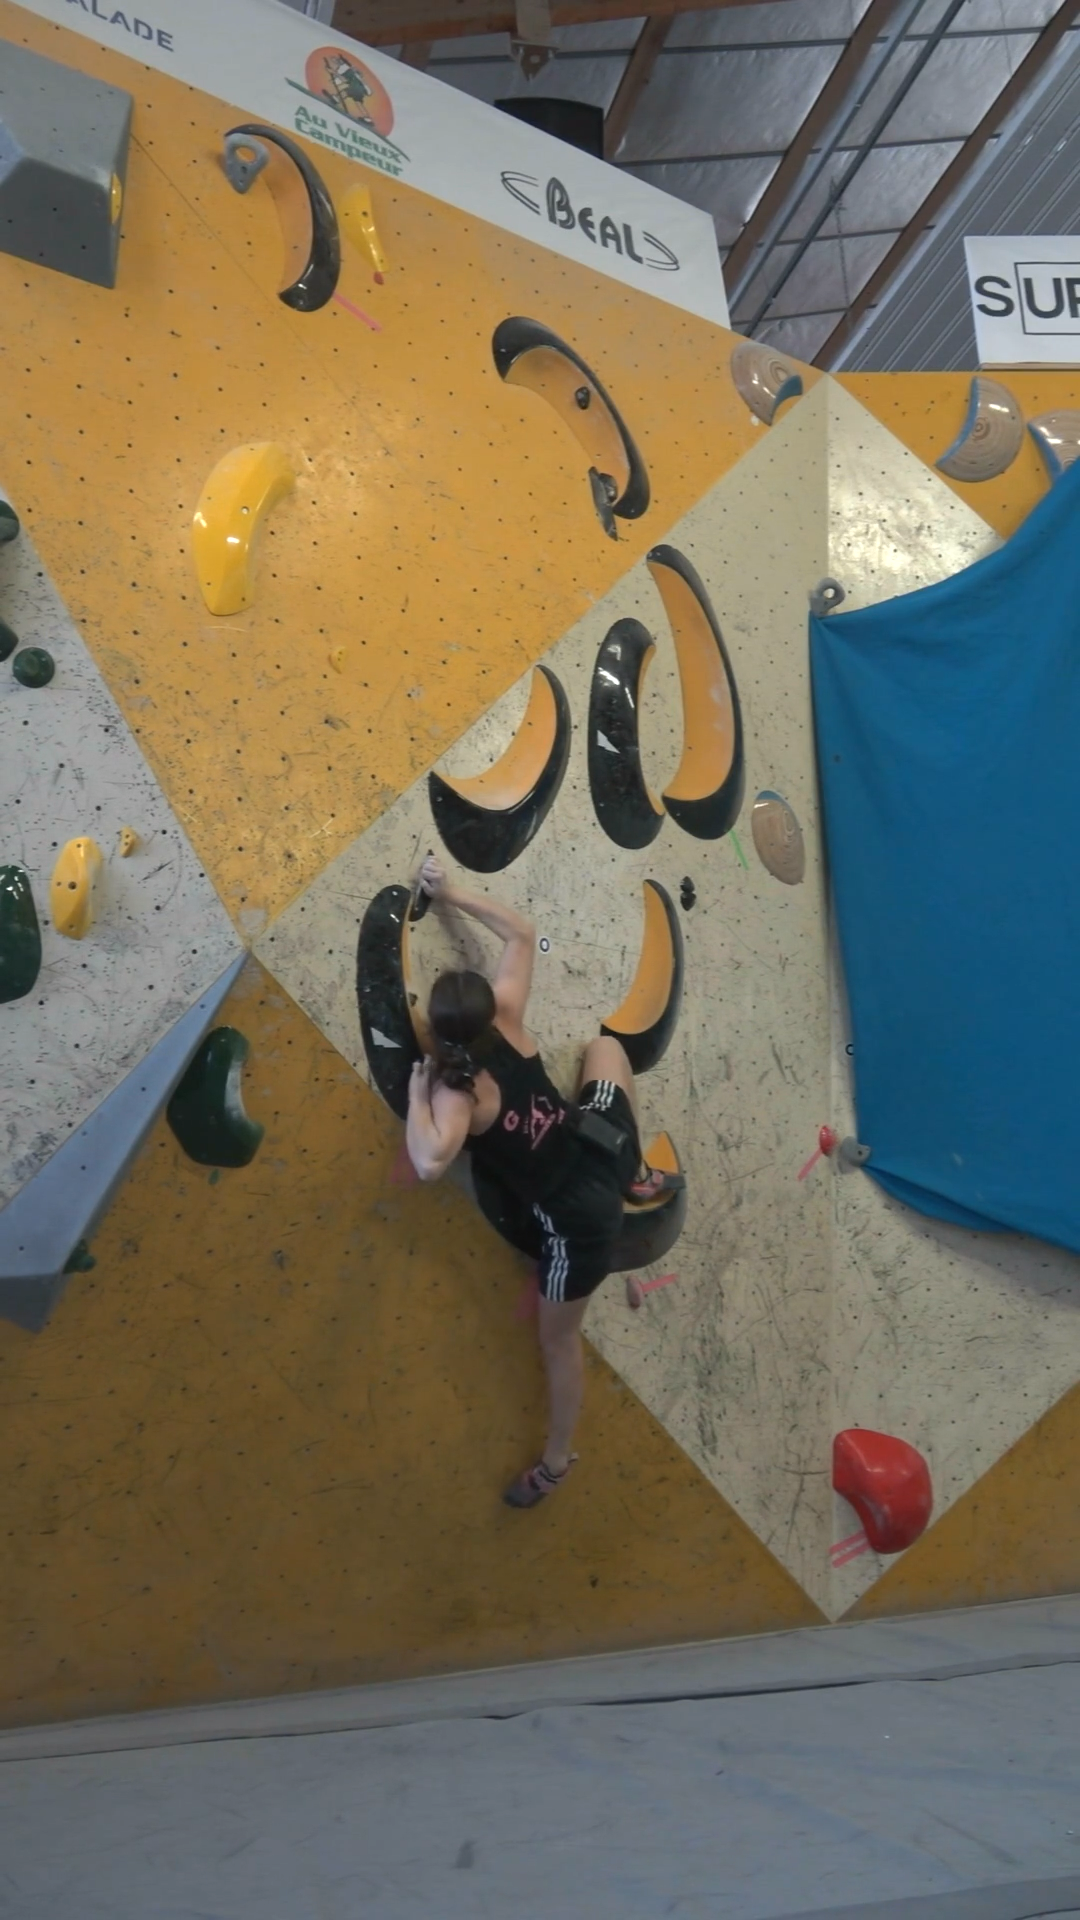
\includegraphics[width=0.2\textwidth]{assets/images/climbing.2.png}} \\[6pt]
      (a) Observing the block. &
      (b) Brushing the grips. &
      (c) Climbing the block. &
      (d) Climbing the block.
    \end{tabular}
    \caption{Different phases of bouldering.}
    \label{fig:phases-of-bouldering}
  \end{figure*}
\section{Problem Setup}

\begin{tcolorbox}[colback=lightgray!10, colframe=black, title={Research Aim}]
    This project focuses on the task of temporal action segmentation in professional bouldering videos. The goal is to classify each frame based on the climber's activity, enabling a more detailed analysis of the climber's performance throughout the video.
\end{tcolorbox}

\subsection{Video Representation}
We represent each video as a sequence of frames $video_i = \{f_1, f_2, \dots, f_{N_i}\}$, where each frame $f_i$ corresponds to the image captured at position $i$ in the video. Each frame $f_i$ is a tensor with shape $(3 \times H \times W)$, where $3$ denotes the number of channels, $H$ is the height of the video, and $W$ is the width of the video. The total number of frames in the video is denoted by $N_i$.

The $i$-th video's duration, $d_i$, in seconds is given by $d_i = N_i / F$, where $F$ is the frame rate of the video. In our experiments, we fix $F = 25 \, \text{fps}$, which matches the frame rate used in our dataset.

\subsection{Annotation Representation}  
Each video's annotations are provided at the frame level. Given a video $video_i$, its corresponding annotations are defined as $a_i = \{c_1, c_2, \cdots, c_{N_i}\}$, where $c_j \in C$ is the annotation corresponding to the frame $f_i$, and $C = \{\text{Climbing, Brushing, Observing, Stopwatch}\}$ is the set of all possible activity labels.

Alternatively, the annotations can be represented using start and end timestamps. In this format, the annotations are defined as a set of tuples:  
\[
\{(s_1, e_1, c_1), (s_2, e_2, c_2), \dots \}
\]  
where $s_j$ is the index of the starting frame for the $j$-th action segment, $e_j$ is the index of the ending frame, and $c_j \in C$ is the corresponding action label.

Depending on the context, the starting frame $s_j$ and ending frame $e_j$ can alternatively be expressed as timestamps (e.g., seconds, milliseconds) or as a starting timestamp combined with a duration. 

This alternative representation is more compact and especially useful when dealing with longer videos or when visualizing action intervals and it is the preferred format when annotating videos as it is easier to deal with. While the first representation provides more precision at the frame level, the second representation offers a higher-level view of the video’s structure, facilitating analysis of action segments and their durations.

Note that it is easy to convert between these two representations by computing the starting and ending frames from the timestamps and vice versa.

\subsection{Problem Formulation}
The goal is to develop a model $\mathcal{M}$ that takes a sequence of frames as input and predicts the corresponding sequence of frame-level annotations, $\mathcal{M}: \{f_1, f_2, \dots, f_{N_i}\} \rightarrow \{c_1, c_2, \dots, c_{N_i}\}$.

\noindent\textbf{Frame-wise Prediction.}  
In this formulation, the model processes each frame independently and predicts its corresponding label. As the each frame is passed through a convolutional layer or a similar architecture. The model predicts a label $c_j$ for each frame $f_j$, i.e.,

\[
c_j = \mathcal{M}(f_j)
\]

While this approach is computationally efficient, it may struggle to capture temporal dependencies between consecutive frames.

\noindent\textbf{Sequence-based Prediction.}  
Here, the model processes a sequence of $T$ consecutive frames and predicts a single label for the entire sequence. A larger segment length $T$ allows the model to leverage more temporal context, improving its ability to recognize complex patterns. This can be expressed as:

\[
c_{j:j+T-1} = \mathcal{M}(f_j, f_{j+1}, \dots, f_{j+T-1})
\]

In this approach, the model predicts the activity label for the entire sequence of frames, taking into account their temporal dependencies. However, this comes at the cost of increased computational complexity.

The choice between these approaches depends on the desired trade-off: a smaller segment length favors computational efficiency, while a larger segment length enhances the model's capacity to capture temporal dependencies. In the following $T$ is taken between $4$ and $32$ frames depending on the model's variant.

\subsection{Additional Statistical Measures}

Besides the usual statistics, such as the mean and average duration, we also utilize the following two metrics, introduced in \cite{tas-survey}, to gain further insights into the data:

\noindent\textbf{Repetition Score.}  
It quantifies the degree of repetition of actions within a video. Using the notations defined earlier, it is expressed as:  

\[
\text{Repetition Score} = \frac{|\{c_j \mid c_j \in a_i\}|}{|a_i|}
\]

where \( |\{c_j \mid c_j \in a_i\}| \) denotes the number of unique action labels in the annotation sequence \( a_i \), and \( |a_i| \) represents the total number of annotated actions in the video. This score ranges from 0 to 1, where 0 indicates no repetition of actions, and 1 indicates that the same action is repeated throughout the video.

\noindent\textbf{Order Variation Score.}  
It measures the consistency of the order of actions across different videos or sequences. Using the previously defined notations, it is expressed as:  

\[
\text{Order Variation Score} = \frac{1}{|V|} \sum_{i, j \in V} d(a_i, a_j)
\]

where \(d(a_i, a_j)\) represents the pairwise distance between the annotation sequences \(a_i\) and \(a_j\), and \(V\) is the set of all videos in the dataset. The score ranges from 0 to 1, where 0 indicates identical action order across all videos, and 1 indicates completely inconsistent action order.  

\subsection{Evaluation Metrics}

During the project we are going to use the \textbf{Accuracy} as a metric to evaluate the model's performance. It is defined as:

$$
\text{Accuracy} = \frac{\text{Correct Predictions}}{\text{Total Predictions}}.
$$
\noindent\textbf{\small{Pros.}} Simple to compute and provides a clear overall performance indicator. \textbf{\small{Cons.}} Not informative for imbalanced classes, as high accuracy can be achieved by predicting the majority class.

\begin{AIbox}{Pyhton Package - TAS Helpers.}
    We introduce the \texttt{tas\_helpers} (Temporal Action Segmentation Helpers) library, which contains implementations of various metrics and scores discussed above. Additionally, it offers utilities for visualizing video segmentations and more. The package is available at: \url{https://github.com/raideno/tas-helpers}.
\end{AIbox}

\begin{figure*}[t]
  \centering
  \begin{tabular}{@{}cccc@{}}
    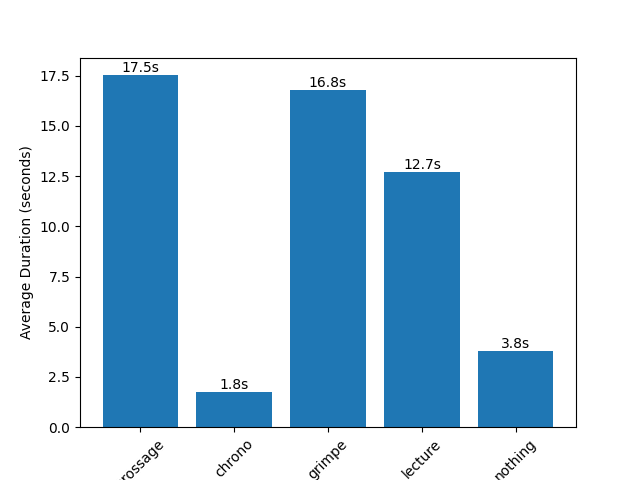
\includegraphics[width=0.23\textwidth]{../../assets/figures/average-duration-of-actions.png} &
    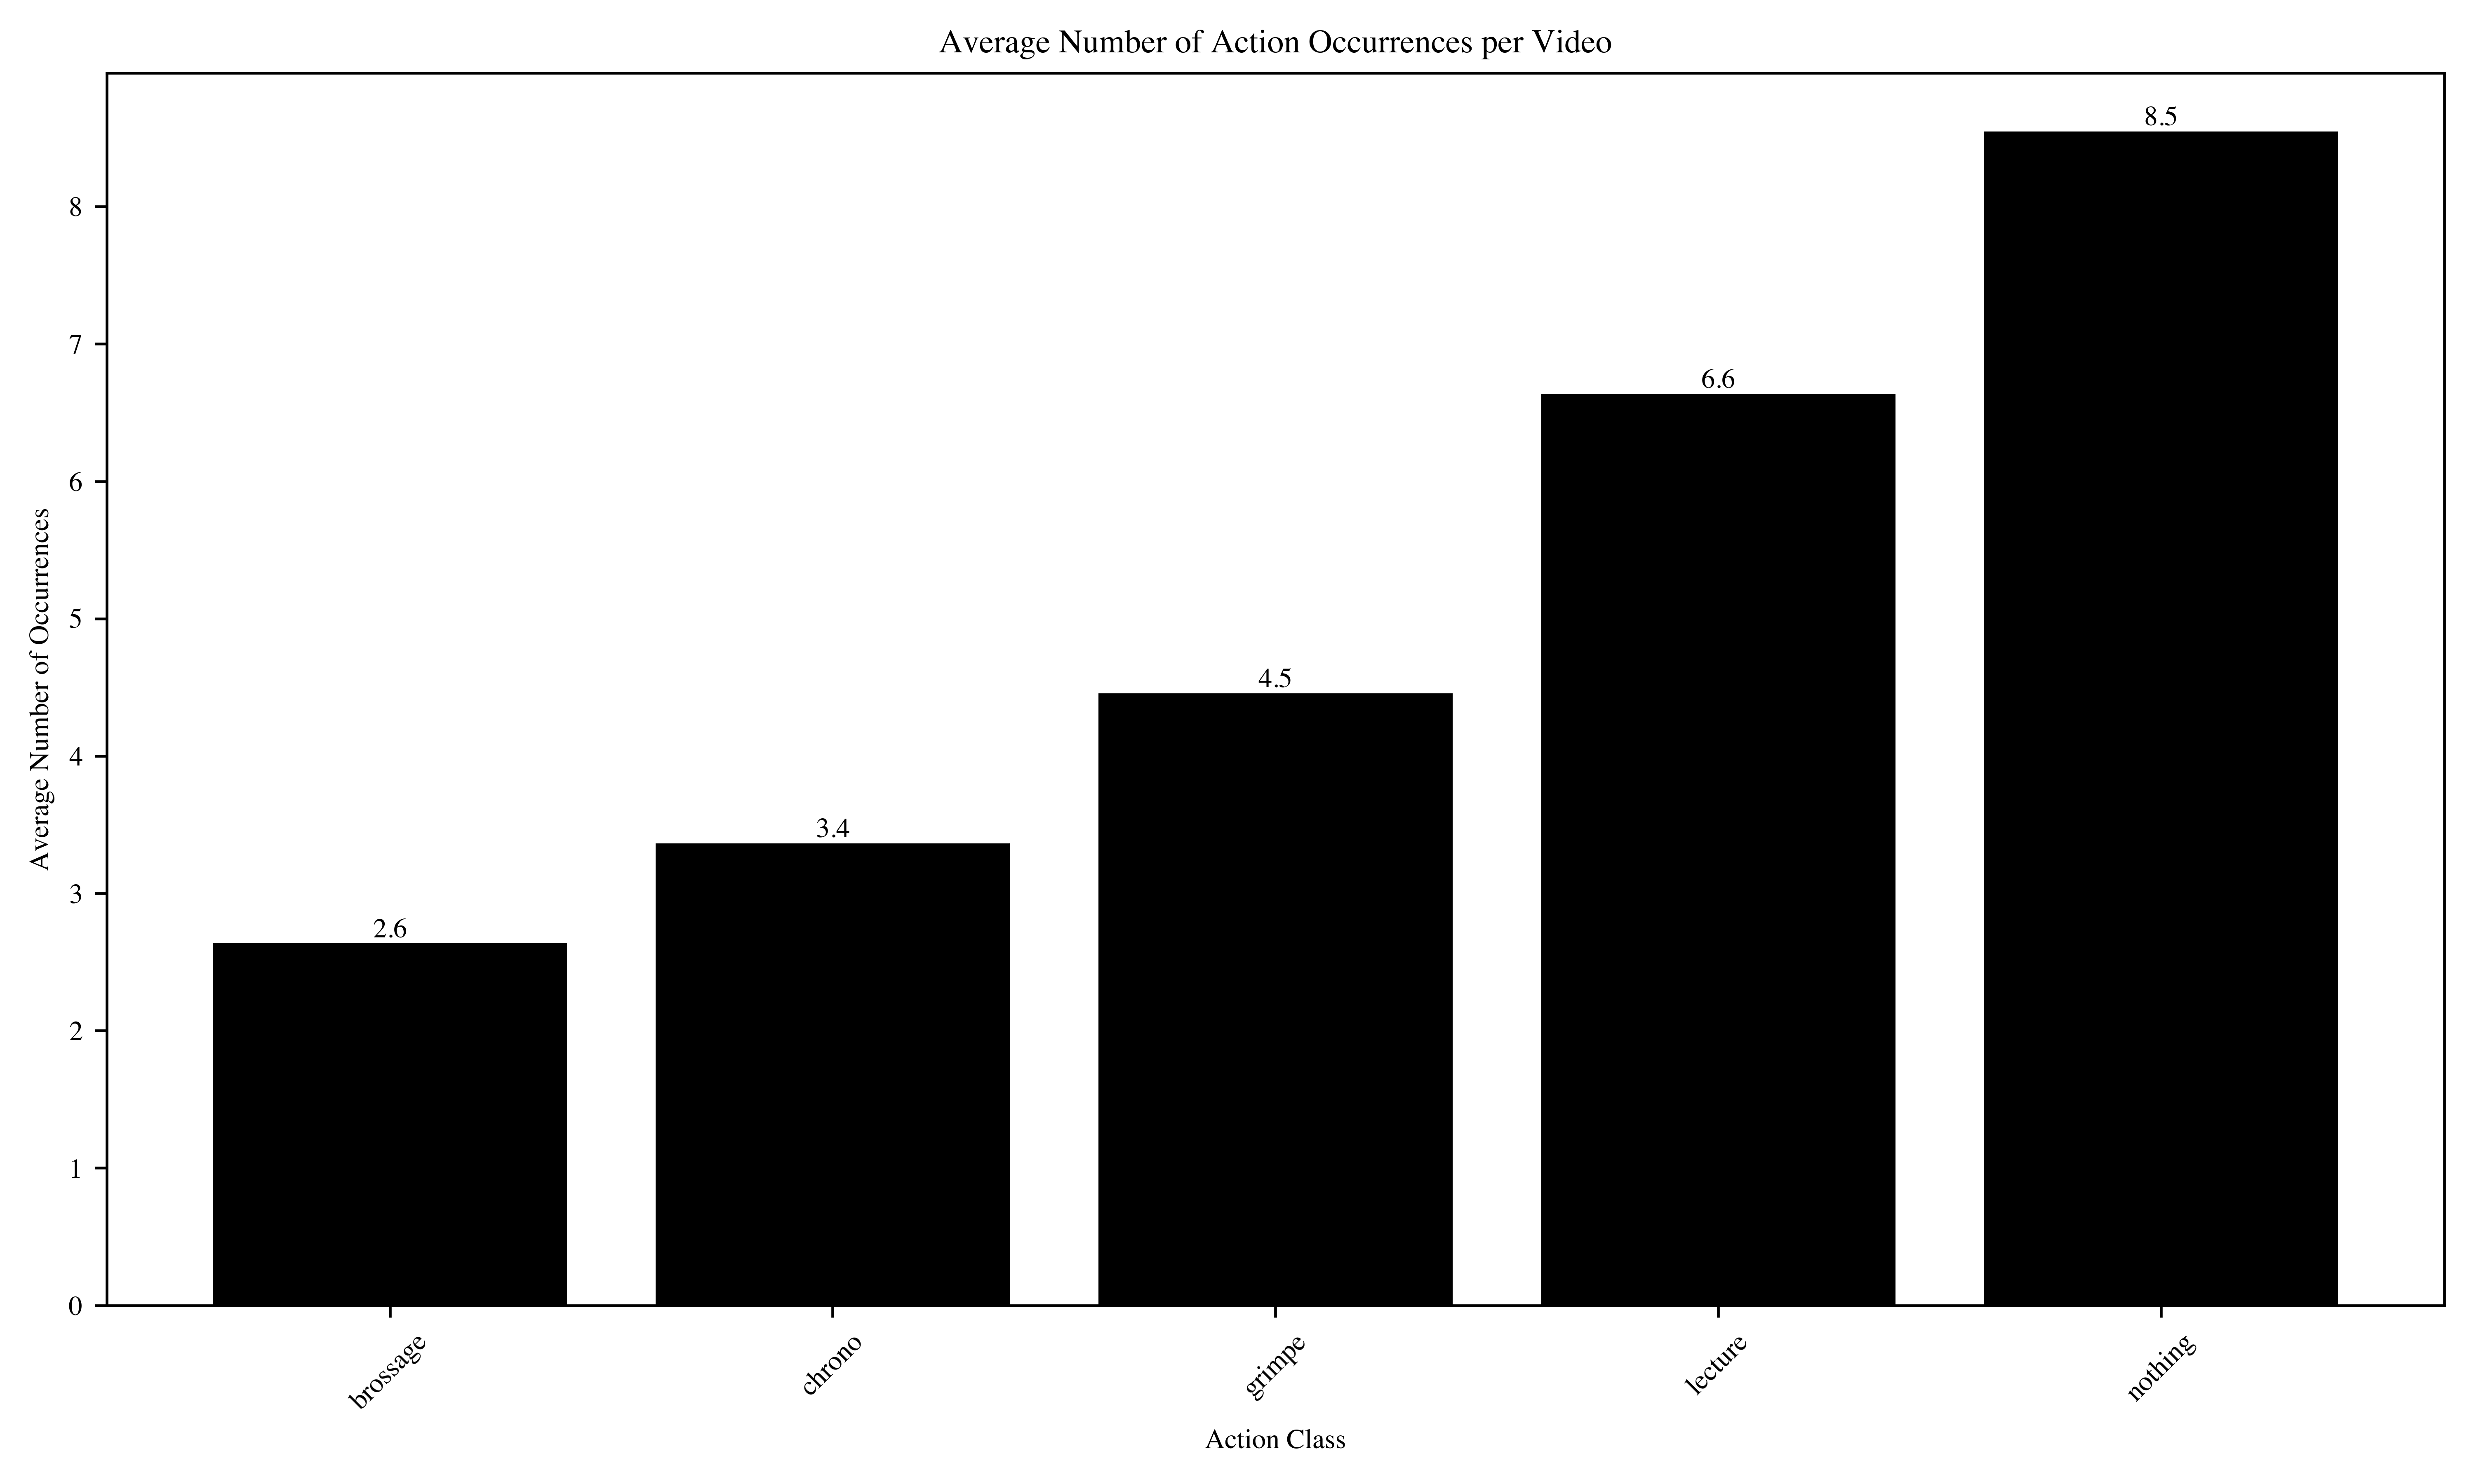
\includegraphics[width=0.23\textwidth]{../../assets/figures/average-number-of-action-occurrences-per-video.png} &
    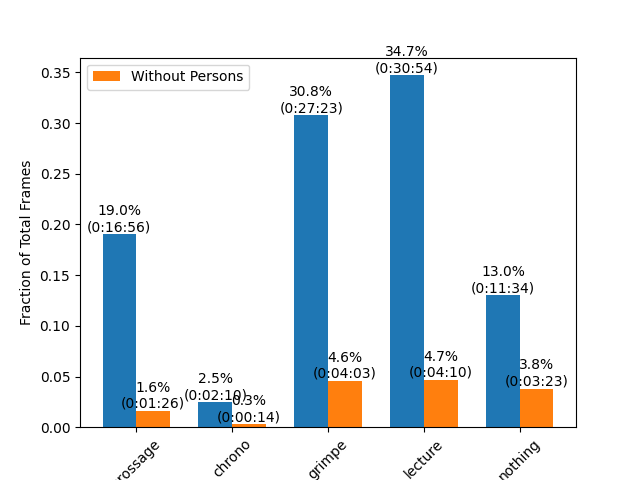
\includegraphics[width=0.23\textwidth]{../../assets/figures/distribution-of-actions-in-dataset.png} &
    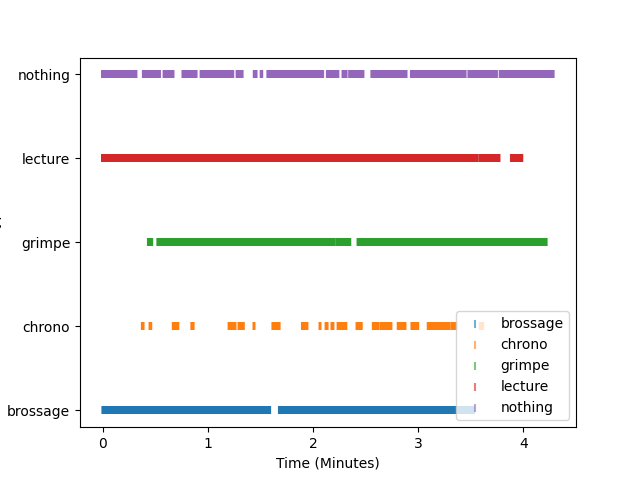
\includegraphics[width=0.23\textwidth]{../../assets/figures/temporal-distribution-of-actions.png} \\
    \begin{minipage}{0.23\textwidth}\centering\caption{Average duration of actions in the dataset.}\label{fig:average-duration-of-actions}\end{minipage} &
    \begin{minipage}{0.23\textwidth}\centering\caption{Average Action Count per Video.}\label{fig:average-number-of-action-occurences-per-video}\end{minipage} &
    \begin{minipage}{0.23\textwidth}\centering\caption{Distribution of actions in the dataset.}\label{fig:distribution-of-actions-in-dataset}\end{minipage} &
    \begin{minipage}{0.23\textwidth}\centering\caption{Temporal distribution of actions in the dataset}\label{fig:temporal-distribution-of-actions}\end{minipage}
  \end{tabular}
\end{figure*}

\section{Dataset}

In this section, we present the dataset used in this project, detailing its construction, preparation, and some important statistics. We also compare our dataset to other popular datasets used in temporal action segmentation.

\subsection{Raw Format}

Our dataset was collected during the "Manip Chambery" bouldering event. It consists of videos filmed from two different angles of 10 climbers attempting to complete 2 distinct bouldering blocks (events) each. This resulted in a total of 20 unique climbs, or 40 videos in total, with each video having a duration of 4 minutes.

The climbers' activities during the event are diverse. They may engage in actions such as brushing the holds, observing them, and climbing. These actions occur freely within the 4-minute duration of each video, providing a rich set of diverse activities.

As specified in \cite{section:context}, the videos were annotated by the climbers themselves, and the annotations were provided in raw Excel format. The annotations are segment-level, meaning that for each action, we are given the start time and duration of the activity, along with the corresponding label. Out of the 20 climbs, 11 have been annotated with action segments.

The total duration of the dataset is 2 hours and 40 minutes, of which 1 hour and 28 minutes are annotated, forming the basis of our experiments.

\noindent\textbf{Dataset Limitations.}  
While the dataset provides valuable data for action segmentation tasks, it has several limitations: 

\textbf{1.} The dataset size is relatively small, containing only 40 unique videos.
\textbf{2.} The annotations are provided in Excel format, which is not ideal for modern data science workflows.
\textbf{3.} The annotations themselves are not perfect, as they may be shifted in time, and the videos do not always start precisely at the beginning of the event.
\textbf{4.} Climbers occasionally leave the frame during the video, and in some instances, other people may enter the frame, which introduces noise to the data.

Despite these limitations, this dataset provides an essential foundation for the development and evaluation of action segmentation models in the context of bouldering.
\subsection{Chosen Structure}

We decided to structure the dataset in a way that is specifically suited for temporal action segmentation and classification tasks, with a focus on both ease of use and efficiency for training. This structure is designed to allow for easy scalability as new data is added to the project, an important consideration as the dataset will be updated by individuals who may not have a background in data science.

\begin{verbatim}
    dataset
    +-- videos
    |   +-- video-1
    |   |   +-- frame-1.jpg
    |   |   +-- frame-2.jpg
    |   |   +-- ...
    |   +-- ...
    +-- annotations
    |   +-- video-1.csv
    |   +-- video-2.csv
    |   +-- ...
\end{verbatim}

The advantage of this structure is that it does not require additional processing of the videos or annotations provided by the data collection team, ensuring the dataset can be easily expanded with new annotations or videos in the future.

To optimize for video loading, we store each video as a sequence of JPG frames rather than the video file itself. This avoids the need for decoding during runtime, though it comes at the cost of additional storage space. This structure also makes the dataset more versatile and compatible with various libraries and tools.

\begin{AIbox}{Python Package - Video Dataset.}
  We have developed a Python package, \href{https://github.com/raideno/video-dataset}{https://github.com/raideno/video-dataset}, to support this dataset structure. The package provides utilities for easily loading videos, transforming them into this frame-based format, and handling annotations at the frame level. It is highly customizable and can be adapted to work with different types of datasets.
\end{AIbox}

A related tool, \href{https://github.com/raideno/cached-dataset}{https://github.com/raideno/cached-dataset}, serves as a wrapper for an existing dataset, caching the transformed version on disk. This is particularly useful in avoiding the need to repeatedly extract features during model training or evaluation. We will discuss the details of this tool in the training procedure section.

By utilizing this structure and the provided tools, we were able to quickly load the dataset and begin training the model.

\subsection{Data Exploration}

In this section we are going to explore various aspects and statistics about our dataset.

As the plot in Figure \ref{fig:distribution-of-actions-in-dataset} shows, the dataset contains 5 different actions, with each action occurring a different number of times. The distribution of actions is not uniform, with some actions appearing more frequently than others. This non-uniform distribution can be challenging for the model to learn, as it may lead to biases in the predictions. The dataset is unbalanced

\todo[inline]{Explain the plotst.}

We can also see that a significant portion of the dataset (15\%) frames don't contain any person in the frame. We can also observe that 3\% of the time there is more than one person in the frame which can be a source of noise for the model.
\todo[inline]{Add the plot that talks about the percentage of frames with more than 1 peron.}
In addition to that we can see that 13\% of the climbs are not annotated at all and we thus replaced it by a "Nothing" label.

From \ref{fig:average-number-of-action-occurences-per-video} we  can see that the most recurrent actions are "Lecture" and "Nothing".

From the \ref{fig:average-duration-of-actions} we can see that the longest actions on average are the cleaning, climbing and observation. Even tho the nothing class is the most recurrent it is the shortest in duration on average.

\subsection{Popular Video Datasets}

\label{subsection:popular-video-datasets}

\begin{figure}[h!]
    \centering
    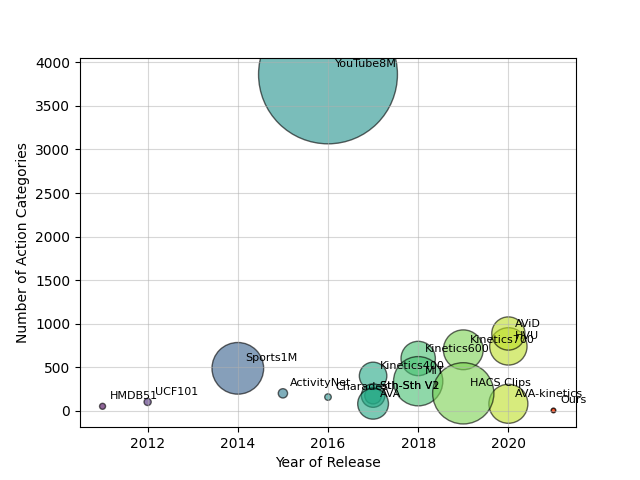
\includegraphics[width=1\linewidth]{../../assets/figures/popular-datasets.png}
    \caption{A visualization of popular video datasets.}
    \label{fig:your-label}
\end{figure}

While there are a number of video datasets available for action recognition and segmentation tasks, the overall number remains limited compared to image or text datasets. Video datasets are much more complex due to the added temporal dimension, and therefore require a significantly larger number of samples for effective model training. For instance, while image datasets might need millions of samples, video datasets typically require tens of millions of samples due to the increased complexity.

Some of the most notable video datasets designed for temporal action segmentation include:

\noindent\textbf{50 Salads Dataset.} This dataset features videos of people preparing salads, focusing on fine-grained hand interactions with the environment \cite{50salads-dataset}.

\noindent\textbf{GTEA Dataset.} Consists of Point of View (POV) videos of food preparation, capturing various sub-actions \cite{gtea-dataset}.

\noindent\textbf{Breakfasts Dataset.} Videos of breakfast preparation, with a focus on fine-grained action segmentation \cite{breakfast-dataset}.

\noindent\textbf{Kinetics Family.} Large-scale datasets containing YouTube clips of various human actions, ranging from sports to human-object interactions \cite{kinetics-400-dataset}, \cite{kinetics-600-dataset}, \cite{kinetics-700-dataset}.

\noindent\textbf{Assembly101 Dataset.} Videos of people assembling and disassembling objects, captured from multiple angles, including some POV \cite{assembly101-dataset}.

\noindent\textbf{HowTo100M Dataset.} A massive dataset of instructional (tutorial) videos, covering a broad range of activities \cite{howto100m-dataset}.

\noindent\textbf{Something-Something V2.} Videos of basic actions such as picking up a pen, captured from a POV perspective, focusing on fine-grained interactions \cite{something-something-dataset}.

Note that the three first datasets were specifically designed for temporal action segmentation.

\begin{table}[!h]
    \centering
    \small
    \resizebox{1\linewidth}{!}{
    \begin{tabular}{lcrr}
    \toprule
    Dataset & Release Year & \#Samples & \#Actions \\
    \midrule
    HMDB51 & 2011 & 7000 & 51 \\
    UCF101 & 2012 & 13300 & 101 \\
    Sports1M & 2014 & 1100000 & 487 \\
    ActivityNet & 2015 & 28000 & 200 \\
    YouTube8M & 2016 & 8000000 & 3862 \\
    AVA & 2017 & 385000 & 80 \\
    \multicolumn{1}{c}{\vdots} & \multicolumn{1}{c}{\vdots} & \multicolumn{1}{c}{\vdots} & \multicolumn{1}{c}{\vdots} \\
    MIT & 2018 & 1000000 & 339 \\
    HACS Clips & 2019 & 1550000 & 200 \\
    HVU & 2020 & 572000 & 739 \\
    AViD & 2020 & 450000 & 887 \\
    \midrule
    \textbf{Ours} & 2024 & 22 & 4 \\
    \bottomrule
    \end{tabular}
    }
    \vspace{-2ex}\caption{A list of popular video datasets.}
    \end{table}
\section{Related Work}

\begin{figure*}[t]
    \centering
    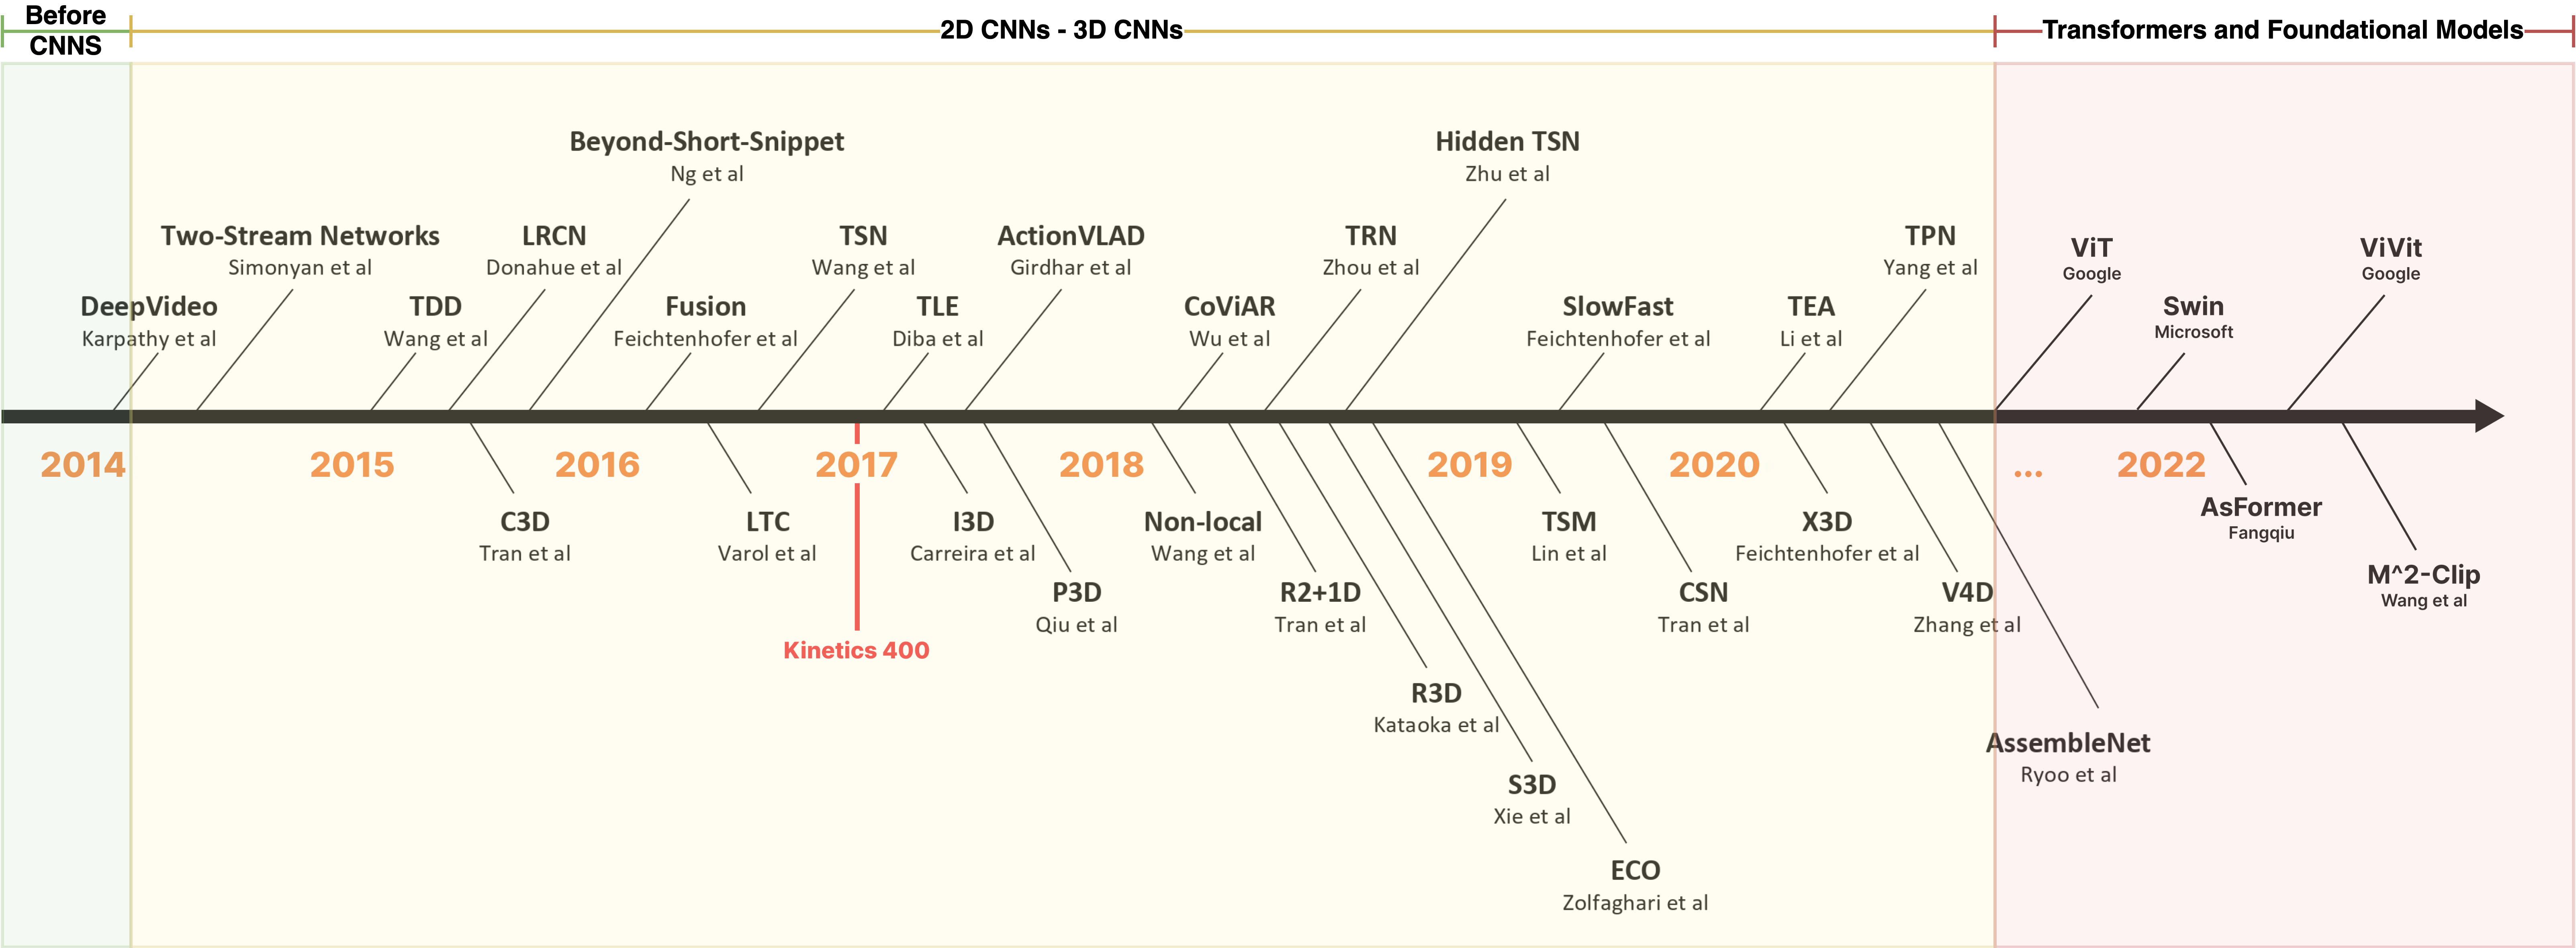
\includegraphics[width=\textwidth]{../../assets/figures/extended-video-timeline-v3.png}
    \caption{A timeline overview of the evolution of video analysis models.}
    \label{figure:video-models-evolution}
    \cite{video-action-recognition-study}
\end{figure*}

In this section, we explore some of the prominent approaches to temporal action segmentation (TAS), discussing how methods have evolved over time as computational power and dataset availability have increased.

\subsection{The Evolution of Video Analysis Models}

The development of video analysis models has seen a significant shift as computational power and dataset size have increased. Initially, video analysis relied heavily on hand-crafted feature extraction \cite{handcrafted-features-1,handcrafted-features-2}, where specific features such as pixels were manually chosen or extracted. With the introduction of optical flow, models began incorporating motion information \cite{i3d}, improving their ability to understand temporal sequences in videos.

As 2D Convolution Neural Networks (CNNs) gained popularity, they were applied to video data for feature extraction, showing promising results for action recognition \cite{tsn}. Following this, the introduction of 3D Temporal CNNs \cite{s3d,resnet-3d,x3d,i3d,slowfast} allowed for better understanding of the temporal dimension in videos. These methods, combined with the advent of larger datasets like Kinetics \cite{kinetics-400-dataset} and Something-Something \cite{something-something-dataset}, marked a turning point in video action recognition, leveraging deep learning to handle complex temporal and spatial patterns in video data.

In recent years, transformers have also emerged as a promising approach for video analysis. Initially used for NLP tasks, transformers have demonstrated strong potential for video action recognition \cite{vivit,dinov2,action-clip}. However, unlike CNNs, transformers lack strong inductive biases \cite{vit}, such as locality and translation invariance, which CNNs excel at. This makes transformers more dependent on massive amounts of data to perform effectively.

The increasing availability of video datasets and computational resources has catalyzed these developments, enabling more sophisticated models. However, video models still face significant challenges due to the vast and diverse distribution of video data. This distribution causes models to drift more rapidly compared to other data types, which makes generalization across different datasets more difficult. Consequently, large datasets are essential for training video models, and pre-trained models often struggle to generalize beyond their original training sets. Moreover, networks with a large number of parameters are particularly prone to overfitting when trained on smaller datasets \cite{resnet-3d}.

\subsection{Temporal Action Segmentation and Its Approaches}

Temporal Action Segmentation can be approached in several ways. Here, we explore a few key perspectives \cite{tas-survey}:

\noindent\textbf{1. Video Classification.} In video classification, the focus is on assigning a single action label to an entire video or segment, typically using models such as 2D or 3D CNNs. This is the most popular perspective in the field, with well-established pre-trained networks available for various datasets. 

\noindent\textbf{2. Temporal Action Detection / Localization.} In this approach, the goal is to detect the temporal boundaries of actions within a video. This task is more challenging than video classification as it requires the model to identify both the start and end of actions while also classifying them.
\begin{figure*}[t]
    \centering
    \begin{minipage}{0.49\textwidth}
        \centering
        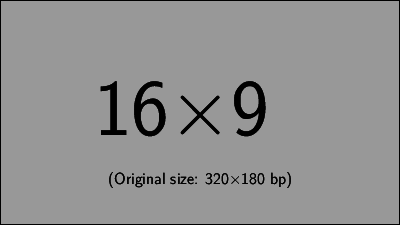
\includegraphics[width=\textwidth]{assets/mwe/example-image-16x9}
        \caption{Local Temporal Modeling}
        \label{figure:local-temporal-modeling}
    \end{minipage}
    \hfill
    \begin{minipage}{0.49\textwidth}
        \centering
        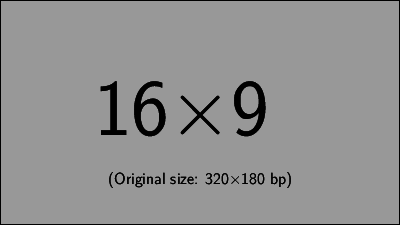
\includegraphics[width=\textwidth]{assets/mwe/example-image-16x9}
        \caption{Global Temporal Modeling}
        \label{figure:global-temporal-modeling}
    \end{minipage}
\end{figure*}

\section{Our Approach}

Given the dataset size constraint we are faced with, it is obvious that training a neural network from scratch only with our data is completely infeasible and wouldn't yield any results.

This is why we took the decision to profit from networks that are pre-trained on popular huge datasets that ressembles the kind of actions available in ours and thus profit and take advantage of the features learned by this networks. In simple words the idea is to take pre trained networks and extract the representation they make of our videos, clips, frames in their hidden layers and use it for classification by passing it into another network we would make.
The idea is that this network we are going to use as a backbone for sure contains some relevant features that understand the video teporality and sptiality in some way and this features must contains enough information about the video segment to do some sort of classification such as for the kinetics dataset, and thus we'll try to extract this information and use it in order to classify on our custom classes. 

In addition to minimizing the damage made by the dataset constraints, taking this approach also reduces the required computational power as it is limited in our case, since we are not training a big network from scratch. And on top of that designing a neural network architecture would require more expertise and time (only 120 hours for the research project) which i don't have yet.

\begin{figure*}[t]
    \centering
    \begin{minipage}{0.49\textwidth}
        \centering
        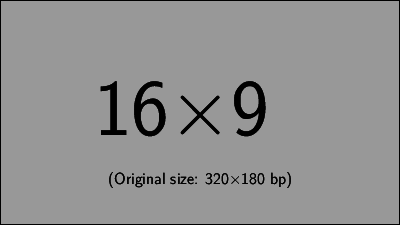
\includegraphics[width=\textwidth]{assets/mwe/example-image-16x9}
        \caption{Illustration of our Model}
        \label{figure:local-temporal-modeling}
    \end{minipage}
\end{figure*}

\subsection*{Considered Variants}

As the temporal context window of the backbone networks is quite limited to around 16-32 frames usually, processing the whole 4 mins of video and extracting a single feature for the whole video is both computationally costly and not practical in our case (would be practical for video classification) since we want to extract the different time segments and classify them rather than classifying the whole video.
This is why we present two approaches.

\subsection{Local Temporal Modeling}
It is called like that as we take a video segment of N frames (N depend on the backbone model being used), extract the features from it and use this features to perform classification.
This method is quite straightforward and easy to implement but the main issue is that we are ignoring the fact that the small video segments belong to the same video, as the classification model 
can maybe benefit from that and maybe some actions only happen at certain moments of the climb, this can also reduce and prevent the noise in classes as the model wouldn persist a class in time rather than keeping it only for 32 frames.

\todo[inline]{Talk about positional embedding.}
\todo[inline]{Reference the figure.}

\subsection{Global Temporal Modeling}

\todo[inline]{Talk about the possible use of attention in this case and how it affects the performance, maybe it allows the model to only focus on the last frames which is the most important ?}

In order to achieve that we are going to use an LSTM for the classification network rather than an MLP. We keep the LSTM very simple and lightweight with only a single layer just like the MLP in order to avoid overfiting given our dataset size.

\todo[inline]{Reference the figure.}

\subsection*{Feature Extractors}
Multiple options are available for the backbone model that will perform feature extractions, we can distinguish two types: Frame Level Feature Extractor and Segment / Video Level Feature Extractor.

\todo[inline]{Talk about temporal sub sampling and justify it's use by the dears of the papers in the field that says it is very efficient and that it reduces computations a lot and that it is trivial and logique to think that it won't drop performance as there isn't a lot of change betwen two consecutive frames.}

\textbf{Frame Level Feature Extractor}
This can essentially be any model that extract some features given a frame, it can be a 2D CNN model such as 2D ResNet, etc, a Vision Transformer such as Deno, Clip, Google ViT, etc or some custom handmade features such as using Yolo keypoints or positions or presente of certain objects such as a brush, elevation of the climber, etc.

This type of feature extractor is very convenient as pre-trained image feature extractors are very abundant as many years have passed through the subject and enough time for it to murir.

Extracting custom features can be tricky and hard to do, for example we could check whether a brush is present on the frame or not and if it is close to the climber, while this is a good idea the thing is that the brush can take different forms in different climbing competition and isn't necesarily a brush, on top of that this requires training a networ for object detection which is costy both in data and computation which are two things we don't have.

Thus we'll mainly stick to the automatic feature extractors during this study.

A question arise from  the frame level feature extractors which is how to combine the frames features into a single feature representing the clip / segment of the video from which the frames have been taken ?

We can distinguish three main possibilities:

The first one is to concatenate the different features forming a single big one, this is the easiest method but not convinient at all as it can form big vectors that don't necessarily have sense.

The second one would be to average (or add them) the different features of the frames and come up with a single one. Doing that for the YOLO model would be just like taking the average position of the climber during the video segment.
\todo[inline]{Cite that in the deno paper and lot of other ones, it is recommanded that taking the average works well.}

The third one which is the most interesting would be to temporally model (link them) this features using an LSTM (in order to create the temporal dependence and come up with a feature that is temporally aware) in order to come up with a single feature representing the video. This approach is certenly the most interesting one.

The cons of temporal modeling is the introduction of another component into the architecture which complexify it and add parameters.

We could also use some linear layer in order to combine them.

\todo[inline]{Here we'll briefely describe the feature extractors we used and more importantly their types (Frame level, Segment level, Slow fast, etc. The goal isn't to fully detail them as this will be done in the )}

\textbf{Video / Clip / Segment Level Feature Extractor}

This models are usually 3D CNNs that have been created and trained by inflating 2D CNNs with some additional things. More recently Transformers have been employed for this and are working pretty well but the issue with that is the rquireemnt of huge computational power and datasets to compensate the lack of inductive baies which is present in CNNs for example.

Using this type of feature extractor, no further processing is required to be done on the videos.

\subsection{Training - Methodology}

\todo[inline]{Talk about how we setup training}
\todo[inline]{Talk about data filtering and what we have done to improve the results such as removing personless and multi person frames, getting rid of low quality data such as unanotatated rather than puting a nothing label, etc}
\todo[inline]{Talk about the training setup that was used.}
\section{Results}

\begin{table*}[t]
    \centering
    \small
    \resizebox{1\linewidth}{!}{
        \begin{tabular}{lcrr||c|lll||c|lll}
            \toprule
            \multicolumn{4}{c||}{\textbf{Model Information}} 
            & \multicolumn{4}{c||}{\textbf{MLP - Accuracy}} 
            & \multicolumn{4}{c}{\textbf{LSTM - Accuracy}} \\
            \cmidrule(lr){1-4} \cmidrule(lr){5-8} \cmidrule(lr){9-12}
            Backbone & Type & \#Params & \#Frames (Seconds)
            & Overall Accuracy & Brushing Class & Reading Class & Climbing Class 
            & Overall Accuracy & Brushing Class & Reading Class & Climbing Class \\
            \midrule
            yolo & By Frame & 2.9M & 8 (0.32) & 65.84\% ± 3.93 & 33.63\% ± 8.67 & 72.81\% ± 7.96 & 78.87\% ± 6.49 & 70.61\% ± 3.62 & 54.79\% ± 20.18 & 75.30\% ± 9.07 & 80.23\% ± 3.05 \\
            dino & By Frame & 22.1M & 8 (0.32) & 80.53\% ± 5.02 & 51.41\% ± 21.74 & 84.98\% ± 4.91 & 90.68\% ± 4.32 & 82.64\% ± 3.15 & 70.98\% ± 4.63 & 82.68\% ± 7.93 & \textbf{92.76}\% ± 3.45 \\
            clip & By Frame & 151.3M & 8 (0.32) & 77.08\% ± 1.88 & 48.76\% ± 16.31 & 77.66\% ± 9.70 & 91.05\% ± 3.56 & 78.72\% ± 3.04 & 58.30\% ± 10.55 & 85.84\% ± 5.69 & 89.55\% ± 5.02 \\
            \midrule
            r3d & By Segment & 31.6M & 8 (0.32) & 84.15\% ± 4.59 & 63.14\% ± 19.01 & 86.92\% ± 3.79 & \textbf{92.22}\% ± 2.87 & \textbf{86.80}\% ± 3.50 & 83.46\% ± 4.18 & 87.06\% ± 3.67 & 89.71\% ± 5.64 \\
            i3d & By Segment & 12.7M & 16 (0.64) & 77.61\% ± 7.96 & 56.66\% ± 13.86 & 77.69\% ± 6.42 & 89.88\% ± 5.74 & 79.38\% ± 5.68 & 71.62\% ± 5.64 & 75.79\% ± 16.07 & 89.04\% ± 6.34 \\
            x3d-xs & By Segment & 3.0M & 4 (0.16) & 81.64\% ± 3.76 & 62.65\% ± 12.53 & 82.48\% ± 6.19 & 90.58\% ± 4.65 & 84.90\% ± 2.68 & 81.50\% ± 4.99 & 83.73\% ± 3.82 & 89.80\% ± 3.95 \\
            x3d-s & By Segment & 3.0M & 16 (0.64) & 84.89\% ± 4.90 & 69.96\% ± 14.65 & \textbf{88.83}\% ± 3.71 & 88.48\% ± 5.21 & 85.97\% ± 2.84 & \textbf{84.88}\% ± 5.92 & 82.70\% ± 4.17 & 89.97\% ± 5.78 \\
            x3d-m & By Segment & 3.0M & 16 (0.64) & \textbf{85.39}\% ± 4.16 & \textbf{72.03}\% ± 16.10 & 87.13\% ± 4.09 & 90.50\% ± 4.55 & 85.65\% ± 2.22 & 84.00\% ± 9.41 & 84.45\% ± 6.60 & 89.16\% ± 2.85 \\
            x3d-l & By Segment & 5.3M & 16 (0.64) & 84.79\% ± 4.04 & 69.36\% ± 16.20 & 86.55\% ± 3.81 & 91.35\% ± 2.53 & 85.46\% ± 1.47 & 84.26\% ± 6.07 & 84.41\% ± 8.37 & 87.82\% ± 4.21 \\
            s3d-k & By Segment & 7.9M & 16 (0.64) & 78.38\% ± 5.21 & 57.96\% ± 11.23 & 77.66\% ± 11.26 & 89.65\% ± 2.84 & 78.57\% ± 4.06 & 77.65\% ± 4.85 & 73.37\% ± 5.84 & 84.53\% ± 7.77 \\
            s3d-h & By Segment & 7.9M & 16 (0.64) & 59.52\% ± 8.90 & 00.00\% ± 00.00 & 78.96\% ± 7.35 & 76.79\% ± 15.54 & 43.25\% ± 4.74 & 23.56\% ± 34.56 & 42.93\% ± 29.85 & 58.29\% ± 43.94 \\
            slowfast & By Segment & 33.6M & 32 (1.28) & 84.06\% ± 2.94 & 70.79\% ± 12.22 & 85.00\% ± 2.27 & 90.47\% ± 1.33 & 85.16\% ± 1.80 & 79.18\% ± 7.60 & \textbf{88.54}\% ± 6.68 & 87.82\% ± 3.96 \\
            vivit & By Segment & 88.6M & 32 (1.28) & 77.65\% ± 5.19 & 45.44\% ± 14.48 & 81.71\% ± 8.27 & 90.93\% ± 5.70 & 81.46\% ± 2.21 & 72.71\% ± 9.25 & 82.14\% ± 6.72 & 87.14\% ± 5.72 \\
            \bottomrule
        \end{tabular}
    }
    \vspace{-2ex}
    \centering
    \caption{Models Performance Results.}
    \paragraph{
        The duration in seconds is relative to a 25 FPS video. Note that the X3D  models have the same number of parameters but the FLOPs increase between each member of the family.
    }
    \label{table:training-results}
\end{table*}
    

\begin{figure*}[!htb]
    \centering
    \begin{minipage}{0.48\textwidth}
        \centering
        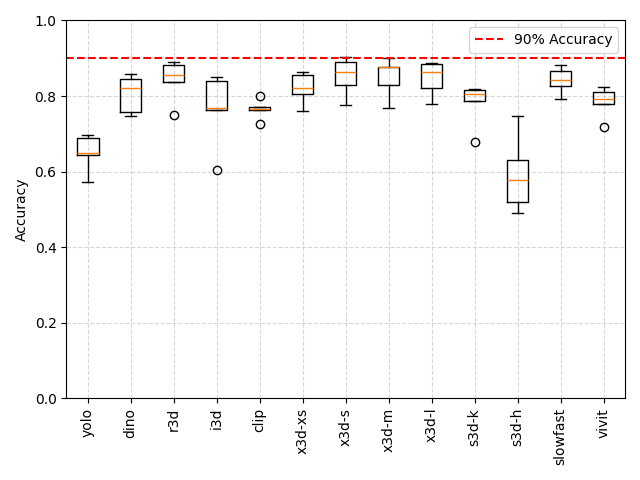
\includegraphics[width=1\textwidth]{../../assets/figures/mlp.training-results.boxplot.png}
        \caption{MLP Model Training Results}
        \label{fig:mlp-training-results}
    \end{minipage}
    \hfill
    \begin{minipage}{0.48\textwidth}
        \centering
        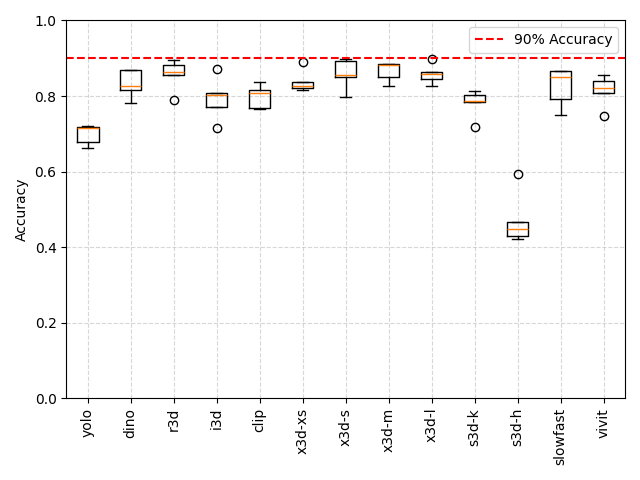
\includegraphics[width=1\textwidth]{../../assets/figures/lstm.training-results.boxplot.png}
        \caption{LSTM Model Training Results}
        \label{fig:lstm-training-results}
    \end{minipage}
\end{figure*}

\subsection{Performance Analysis}
Table~\ref{table:training-results} presents the classification accuracy of various backbone architectures combined with either MLP or LSTM classifiers for bouldering video segmentation. The results reveal several interesting patterns that provide insights into the effectiveness of different approaches for this specific task.

\subsubsection{Segment vs. Frame-based Extraction}
Our experiments demonstrate a clear advantage for models that incorporate temporal information through segment-level processing. As shown in Table~\ref{table:training-results}, segment-based models consistently outperform frame-based models, with the top-performing models (X3D family) all utilizing temporal information. The X3D-S model achieves 85.28\% accuracy with an MLP classifier, while R3D reaches 86.61\% accuracy when combined with an LSTM. This pattern aligns with the intuitive understanding that climbing actions involve temporal dynamics that cannot be fully captured by analyzing individual frames or segments in isolation.

\subsubsection{Analysis of Underperforming Models}
Two backbone architectures exhibit notably lower performance compared to others:

\noindent\textbf{YOLO-based Skeleton Features.}
The YOLO-based approach, which extracts skeletal key points, achieves only 65.01\% accuracy with MLP and 69.94\% with LSTM. This underperformance can be attributed to the similarity in climber movement dynamics across different action categories. For instance, the speed and pattern of movement during observing, brushing, and climbing activities may exhibit similar skeletal motion signatures despite being semantically distinct. A potential improvement would be to incorporate absolute spatial positions rather than positions relative to the climber's center of mass. However, this approach would introduce camera position dependency, potentially reducing generalizability across different recording setups.

\noindent\textbf{S3D with HowTo100M Pre-training.}
The S3D model pre-trained on HowTo100M (S3D-H) shows particularly poor performance (59.37\% with MLP, 47.19\% with LSTM). This can be explained by the nature of the pre-training dataset, which consists primarily of instructional videos featuring fine-grained hand manipulations and subtle movements. The same architecture pre-trained on the Kinetics dataset (S3D-K), which contains more diverse and dynamic whole-body activities, performs substantially better (78.08\% with MLP, 78.04\% with LSTM). This significant performance gap highlights the critical importance of selecting appropriate pre-training datasets that align with the target domain's action characteristics.

\subsubsection{Model Complexity and Performance}
Interestingly, our experiments reveal that larger models do not necessarily yield better performance for this task. The X3D-S model (3.0M parameters) outperforms the larger X3D-L variant (5.3M parameters) when using an MLP classifier. Similarly, the relatively lightweight R3D backbone (31.6M parameters) achieves better results to much larger models such as CLIP (151.3M parameters) and ViViT (88.6M parameters). This suggests that for our specific dataset size and task complexity, model architecture design is more important than raw parameter count. The X3D family, designed specifically for efficient video understanding, demonstrates excellent performance-to-parameter ratios across all variants.

\subsubsection{Temporal Modeling with LSTM}
When comparing MLP and LSTM classifiers, we observe that LSTM generally provides modest improvements across most backbones. For instance, DINO shows a 2.62\% improvement when switching from MLP to LSTM. However, this pattern is not universal—SlowFast actually performs 1.73\% worse with LSTM compared to MLP. The inconsistent benefits of additional temporal modeling through LSTM may be due to our dataset size constraints, as larger datasets typically show more significant improvements from temporal modeling, as demonstrated in prior work \cite{action-clip}.

Beyond improvements in accuracy, we also observe a reduction in variance across multiple runs when using LSTM classifiers. For example, the X3D-M model shows a standard deviation of 4.75\% with MLP but only 2.32\% with LSTM, representing a nearly 50\% reduction in variance. This increased stability is a significant advantage in practical applications, as it indicates more reliable and consistent performance across different climbing sessions and environmental conditions.

\subsection{Practical Implications}
Based on our experimental results, we can draw several conclusions to guide model selection for practical bouldering video segmentation applications:

\noindent\textbf{For accuracy-critical applications.}
The X3D-M with LSTM classifier provides the highest overall accuracy (86.61\%) and represents the best choice when classification performance is the primary concern.
    
\noindent\textbf{For resource-constrained environments.}
The X3D-XS with MLP classifier offers an excellent balance between accuracy (82.11\%) and computational efficiency, utilizing only 3.0M parameters. And this model provide the best trade-off between speed and accuracy.
    
These findings provide valuable insights for climbing gym operators, sports coaches, and performance analysts working with climbing videos. For coaches analyzing technique, the highest accuracy models would better distinguish between different climbing phases, while training facilities with limited computing resources could implement the lighter models for real-time feedback systems. The ability to reliably segment climbing activities enables more targeted training programs and better performance assessment for climbers at all levels.
\section{Limitations \& Future Directions}

While our approach demonstrates promising results for bouldering video segmentation, several limitations remain to be addressed in future work.

\subsection*{Methodological Limitations}
Our current implementation faces several methodological constraints. First, the cross-entropy loss function used may not be optimal for temporal segmentation tasks with class imbalance. Alternative losses could potentially improve performance on underrepresented classes. Second, despite the strong performance of convolution architectures, we did not extensively explore transformer-based approaches specifically designed for video understanding, such as TimeSformer or MViT, which have shown state-of-the-art results in related action recognition tasks.

Real-time processing remains a significant limitation of our current approach. The segment-based models that achieved the highest accuracy operate with inherent latency due to their temporal window requirements. For practical applications coaches usually don't require realtime annotations.

\subsection*{Data-Related Challenges}
Limited training data remains a fundamental constraint. Our dataset, while sufficient to demonstrate the viability of automated bouldering segmentation, lacks the scale and diversity needed for robust real-world deployment. We identify several potential approaches to address this:

\noindent\textbf{Semi-supervised Learning.}
Using our best-performing models to pseudo-label unlabeled climbing videos, then leveraging these annotations for additional training data. This bootstrapping approach could substantially increase our effective dataset size while maintaining a manually verified validation set to avoid bias.

\noindent\textbf{External Data Integration.}
Augmenting training with targeted external data from sources like YouTube or subsets of action recognition datasets like Kinetics that contain climbing or similar activities. This would require careful selection and possibly domain adaptation techniques to ensure relevance.

\noindent\textbf{Data Augmentation.}
While we employed basic augmentation techniques, more advanced video-specific augmentations such as temporal shifts, speed variation, and view synthesis could improve model robustness to variations in climbing styles and camera positions.
\section{Conclusion}

\subsection*{Research Contributions}
This work demonstrates the feasibility of automated bouldering video segmentation using modern deep learning approaches. Our experiments revealed that segment-based models, particularly the X3D family and the R3D, outperform frame-based approaches for this task, achieving accuracies of up to 86.80\%. We established that the choice of pre-training dataset significantly impacts performance, as evidenced by the stark difference between S3D models trained on HowTo100M versus Kinetics. Notably, model complexity did not necessarily correlate with performance, with lighter models often matching or exceeding their larger counterparts.

Future research should focus on improving real-time capabilities, investigating alternative loss functions, and exploring transformer-based architectures for video understanding. Semi-supervised approaches leveraging unlabeled climbing footage could address the data scarcity challenge while maintaining evaluation integrity.

\subsection*{Project Reflection}
This project provided valuable experience in end-to-end data science development. Building a computer vision system from scratch presented numerous challenges, from data collection and annotation to model selection and evaluation. The need to balance performance requirements against computational constraints mirrors real-world AI deployment scenarios.

The most significant challenge was navigating the vast landscape of video understanding models without extensive training resources. This required careful consideration of transfer learning approaches and creative solutions for data augmentation.

This work served as a formative experience in independent research, requiring comprehensive exploration of the computer vision literature and adaptation of techniques across domains. It demanded proficiency across the entire machine learning pipeline—from data preparation to deployment considerations—providing practical skills beyond what typical structured projects offer. This holistic approach to solving a complex visual understanding problem has reinforced both technical capabilities and research methodology fundamentals.

\begin{tcolorbox}[colback=lightgray!10, colframe=black, title={Research Aim}]
    Our goal is to \textit{demystify long chain-of-thought reasoning} in LLMs. Through systematic analysis and ablations, we extract key insights and offer practical strategies to enhance and stabilize its performance.
\end{tcolorbox}
\vspace{-10pt}

\section*{Acknowledgment}
Thanks to \lipsum[10].

% \newpage

\section*{Bibliography}

\bibliography{reference}
\bibliographystyle{icml2025}


\newpage

\bibliography{reference}
\bibliographystyle{icml2025}

\newpage
\appendix
\onecolumn
% You can have as much text here as you want. The main body must be at most $8$ pages long.
% For the final version, one more page can be added.
% If you want, you can use an appendix like this one.  

% The $\mathtt{\backslash onecolumn}$ command above can be kept in place if you prefer a one-column appendix, or can be removed if you prefer a two-column appendix.  Apart from this possible change, the style (font size, spacing, margins, page numbering, etc.) should be kept the same as the main body.

\section{Related Work}
\paragraph{Complex reasoning and chain of thought prompting.} Large Language Models (LLMs) have demonstrated remarkable capabilities in various natural language processing tasks, including complex reasoning. A significant advancement in improving LLM reasoning ability is the implementation of Chain of Thought (CoT) prompting \cite{wei2022cot}. This technique involves guiding models to generate intermediate reasoning steps, thereby improving their performance on tasks that require logical deduction and multistep problem solving. Initial studies \cite{lambert2024tulu, wei2022cot, flan, yu2024metamath} focused on short CoT, where models produce concise reasoning paths to arrive at solutions. Although effective for straightforward problems, short CoT can be limiting when addressing more intricate tasks that necessitate deeper deliberation. OpenAI’s o1 \cite{openai2024o1} series models were the first to introduce inference-time scaling by increasing the length of the CoT reasoning process. This approach helps LLMs tackle complex problems by breaking them into finer steps and reflecting during problem-solving, leading to more accurate and comprehensive solutions. In this work, we explore long CoT by identifying key factors that enable models to exhibit this behavior, encouraging advanced reasoning capabilities.

\paragraph{Reinforcement learning for LLM.} Reinforcement Learning (RL) has proven effective in enhancing LLM performance across domains. RL techniques, such as Reinforcement Learning from Human Feedback (RLHF), align model outputs with human preferences, improving coherence \cite{ouyang2022training}. Recent studies \cite{kimi2025k15, deepseekai2025r1, lambert2024tulu} leverage RL to enable LLMs to explore reasoning paths autonomously for complex problems. DeepSeek-R1 \cite{deepseekai2025r1} achieves strong performance in mathematics, coding, and reasoning tasks without relying on a trained reward model \cite{lightman2023verifystep, wang2024multistep} or tree search \cite{feng2023alphazerolike, snell2024scaling}. Notably, this capability emerges even in base models without supervised fine-tuning, albeit at the cost of output readability. Similarly, Kimi K1.5 \cite{kimi2025k15} enhances general reasoning with RL, focusing on multimodal reasoning and controlling thought process length. These works highlight RL’s role in optimizing reasoning when intermediate steps are hard to supervise, and only final outcomes are verifiable. Our research share a similar setup but with more detail on disentangling how different model behaviors emerge under varying training conditions and initialization strategies.

\newpage
\section{Figures and Tables}

%\begin{figure}[H]
%    \centering
%    \includegraphics[width=1\linewidth]{figs/viz-judge-rule.pdf}
%    \vspace{-20pt}
%    \caption{Downstream task performance when trained on clean data}
%    \label{fig:reward-verifier-clean}
%\end{figure}

\begin{table}[H]
\small
\caption{Performance of model trained with different discount factors for the correctness (cosine) reward and repetition penalty. We see that different reward types have different optimal values.}
\vspace{10pt}
\centering
\begin{tabular}{@{}cccccc@{}}
\toprule
\begin{tabular}[c]{@{}c@{}}Correctness \\ Discount\end{tabular} & \begin{tabular}[c]{@{}c@{}}Repetition\\ Discount\end{tabular} & \begin{tabular}[c]{@{}c@{}}MATH\\ -500\end{tabular} & \begin{tabular}[c]{@{}c@{}}AIME \\ 2024\end{tabular} & \begin{tabular}[c]{@{}c@{}}Theo.\\ QA\end{tabular} & \begin{tabular}[c]{@{}c@{}}MMLU\\ -Pro-1k\end{tabular} \\ \midrule
\multicolumn{2}{c}{SFT} & 50.4 & 3.5 & 20.6 & 32.4 \\ \midrule
\multirow{3}{*}{1.000} & 1.000 & 55.7 & \textbf{5.0} & 25.7 & 34.5 \\
 & 0.999 & \textbf{58.0} & 4.6 & \textbf{26.0} & \textbf{36.5} \\
 & 0.99 & 57.8 & 3.8 & 24.5 & 33.3 \\ \midrule
\multirow{2}{*}{0.999} & 0.999 & 53.5 & 2.1 & 19.5 & 30.7 \\
 & 0.99 & 55.2 & 1.7 & 18.5 & 32.0 \\ \midrule
0.99 & 0.99 & 47.9 & 0.2 & 15.6 & 25.5 \\ \bottomrule
\end{tabular}%
\label{fig:multiple-gamma}
\end{table}

\newpage
\section{Algorithms and Formulas}

\subsection{Cosine Reward Formula}

\begin{equation}
\label{eqn:cosine-lr}
\textbf{CosFn}(t, T, \eta_{min}, \eta_{max}) = \eta_{min} + \frac{1}{2}(\eta_{max} - \eta_{min})(1 + \cos(\frac{t\pi}{T}))
\end{equation}

The formula above is commonly used as the learning rate schedule during gradient descent optimization. It was introduced by \cite{loshchilov2017sgdrstochasticgradientdescent}.

\subsection{N-gram Repetition Penalty}

\begin{algorithm}[H]
\caption{N-gram Repetition Penalty}\label{alg:reward-repetition-penalty}
\begin{algorithmic}[1]
    \STATE {\bfseries Input:} 
    \STATE \ \ \ \ $s$ : sequence of tokens
    \STATE \ \ \ \ $l$ : sequence length
    \STATE \ \ \ \ $N$ : n-gram size
    \STATE \ \ \ \ $P$ : penalty value
    \STATE \ \ \ \ $m$ : maximum sequence length
    \STATE {\bfseries Output:} $r \in \mathbb{R}^m$
    \STATE $seq \gets s[1:l]$ \COMMENT{Extract subsequence of length $l$}
    \STATE $ngrams \gets \emptyset$ \COMMENT{Set of observed n-grams}
    \STATE $r \gets \vec{0} \in \mathbb{R}^m$ \COMMENT{Initialize reward vector}
    \FOR{$j \gets 1$ to $|seq| - N + 1$}
        \STATE $ng \gets (seq[j], seq[j+1], ..., seq[j+N-1])$ \COMMENT{Current n-gram}
        \IF{$ng \in ngrams$}
            \FOR{$t \gets j$ to $j + N - 1$}
                \STATE $r[t] \gets P$ \COMMENT{Apply penalty}
            \ENDFOR
        \ENDIF
        \STATE $ngrams \gets ngrams \cup \{ng\}$
    \ENDFOR
    \STATE {\bfseries Output:} $r$
\end{algorithmic}
\end{algorithm}

\newpage
\section{Extracts}

\begin{tcolorbox}[label=extract:reward-short-term, colback=lightgray!10, colframe=black, title={Short-Term Thinking ($\gamma_c = 0.99$)}]
\textbf{But} in this case, we saw that the fixed points don't satisfy the equation 
\[
p(p(x)) = x.
\]

\textbf{Wait}, maybe the solutions to \( p(p(x)) = x \) are not the fixed points of \( p \), but something else.

\textbf{Alternatively}, perhaps I can consider that \( p(p(x)) = x \) implies that \( p \) is a bijection, 
but since \( p(x) \) is quadratic, it's not necessarily invertible over all real numbers.

\textbf{Wait}, but the problem says that \( p(p(x)) = x \) has four real solutions, so perhaps there are four 
values of \( x \) that satisfy this equation.

\textbf{Alternatively}, perhaps I need to find the roots of 
\[
p(p(x)) - x = 0,
\]
and solve for \( x \). But that seems complicated. Maybe there's a better way.
\end{tcolorbox}

\newpage
\section{Experimental Setup}

\subsection{Evaluation Setup} \label{app:eval-setup}

\paragraph{Benchmarks} Below are details of our evaluation benchmarks:

\begin{itemize}
    \item \textbf{MATH-500} \citep{hendrycks2021math}: an in-domain mathematical reasoning benchmark. MATH consists of 12,500 problems from American high school math competitions. For efficiency, we adopt MATH-500, a widely-used i.i.d. subset of its test split.
    \item \textbf{AIME 2024}: an out-of-domain mathematical reasoning benchmark consisting of the 30 problems from American Invitational Mathematics Examination (AIME) 2024.
    \item \textbf{TheoremQA} \citep{chen2023theoremqa}: an out-of-domain STEM reasoning benchmark consisting of 800 samples. It covers 350+ theorems spanning across Math, EE\&CS, Physics and Finance.
    \item \textbf{MMLU-Pro-1k} \citep{wang2024mmlupro}: an out-of-domain general reasoning benchmark. MMLU-Pro comprises over 12,000 questions from academic exams and textbooks, spanning 14 diverse domains including Biology, Business, Chemistry, Computer Science, Economics, Engineering, Health, History, Law, Math, Philosophy, Physics, Psychology, and Others. For efficiency, we adopt an 1,000-sample i.i.d. subset of its test split, called MMLU-Pro-1k. We tried to keep the distribution identical to the original one. Figure \ref{fig:mmlu-pro-test-downsample} shows the distribution before/after the downsampling.
\end{itemize}

\paragraph{Statistical Metrics} We calculate the average accuracy with at least 4 random seeds. To tame the variance caused by the small size of AIME 2024, we sample 16 responses per prompt.


\end{document}

